\PassOptionsToPackage{hyphens}{url}
\documentclass[11pt,a4paper]{article}

\usepackage[utf8]{inputenc}
\usepackage[spanish,es-nodecimaldot,es-tabla]{babel}
\usepackage[T1]{fontenc}
\usepackage{lmodern}
\usepackage[margin=2.35cm]{geometry}
\usepackage{amsmath}
\usepackage{amssymb}
\usepackage{booktabs}
\usepackage{longtable}
\usepackage{tabularx}
\usepackage{array}
\usepackage{enumitem}
\usepackage{listings}
\usepackage{xcolor}
\usepackage{microtype}
\usepackage{parskip}
\usepackage{titlesec}
\usepackage{hyperref}
\usepackage{graphicx}
\usepackage{caption}
\usepackage{float}
\usepackage{tocloft}
\setlength{\cftsecnumwidth}{2.2em}
\setlength{\cftsubsecnumwidth}{2.8em}

\definecolor{azulWCD}{RGB}{17,67,112}
\definecolor{grisCodigo}{RGB}{247,247,247}
\definecolor{tituloColor}{RGB}{0,55,110}
\definecolor{reglaColor}{RGB}{0,90,160}

\hypersetup{colorlinks=true, linkcolor=azulWCD, urlcolor=azulWCD, citecolor=azulWCD,
  pdftitle={Respuesta electromagnética del WCD a la captura de neutrones: fotones gamma}, pdfauthor={Jaime A. Betancourt}}

\lstdefinestyle{shstyle}{backgroundcolor=\color{grisCodigo}, basicstyle=\ttfamily\footnotesize, breaklines=true,
  frame=single, rulecolor=\color{gray!40}, columns=fullflexible, keepspaces=true}
\lstset{style=shstyle}

\titleformat{\section}{\normalfont\Large\bfseries\color{azulWCD}}{\thesection.}{0.6em}{}
\titleformat{\subsection}{\normalfont\large\bfseries}{\thesubsection.}{0.5em}{}
\setlist{itemsep=0.25em,topsep=0.4em}
\renewcommand{\arraystretch}{1.18}
\setlength{\emergencystretch}{2em}
\captionsetup{font=small,labelfont=bf}
\renewcommand{\cftsecfont}{\bfseries\color{azulWCD}}
\renewcommand{\cftsecpagefont}{\bfseries}

\graphicspath{{../../../analysis/campana-1_respuesta-electromagnetica_seccion-4.2/figuras-gammas/}}
\newcommand{\tablas}{figuras-respuesta-electromagnetica}
\newcommand{\archivo}[1]{\texttt{\detokenize{#1}}}
\newcommand{\var}[1]{\texttt{#1}}

\begin{document}
\pagestyle{empty}

\begin{titlepage}
\begin{center}
\vspace*{0.5cm}
\textcolor{reglaColor}{\rule{\linewidth}{1.2pt}}

\vspace{1.3cm}
{\Large\scshape Universidad Industrial de Santander}\\[0.2cm]
{\large Escuela de Física --- Facultad de Ciencias}\\[0.2cm]
{\large Doctorado en Física}

\vspace{2.2cm}
{\Huge\bfseries\color{tituloColor} Respuesta electromagnética\\[0.3cm] del WCD a la captura\\[0.3cm] de neutrones}

\vspace{1.2cm}
{\Large Fotones gamma}

\vspace{1.4cm}
{\large\textbf{Informe técnico}}

\vspace{0.6cm}
\begin{minipage}{0.82\linewidth}
\centering
\textit{``Producción, interacción y destino de los fotones gamma de captura en agua pura y en agua con NaCl para neutrones de 1~meV a 1~keV: reproducción de la Sección~4.2 de la tesis y verificación del modelo de captura del simulador''}
\end{minipage}

\vfill
{\large\textbf{Autor}}\\[0.15cm]
Jaime A. Betancourt\\[0.1cm]
Doctorado en Física, Universidad Industrial de Santander

\vspace{1.2cm}
\textcolor{reglaColor}{\rule{0.5\linewidth}{0.6pt}}

\vspace{1cm}
6 de octubre de 2026

\vspace{1cm}
\textcolor{reglaColor}{\rule{\linewidth}{1.2pt}}
\end{center}
\end{titlepage}

\pagestyle{plain}

\begin{abstract}
Este informe estudia la respuesta electromagnética del detector Cherenkov de agua (WCD) a la captura de neutrones de la Campaña~1 (dieciséis energías entre 1~meV y 1~keV, agua pura y agua con 2.5, 5 y 10~\% de NaCl, $10^5$ neutrones por corrida, \texttt{QGSP\_BERT\_HP} sin $S(\alpha,\beta)$) en lo que concierne a los fotones gamma: su producción en las cascadas de captura, sus interacciones en el tanque y su destino. Un script del repositorio procesa en once segundos los 64 archivos crudos de fotones (5.07 millones de fotones) y un notebook regenera las figuras gamma de la tesis. La reconstrucción de las cifras publicadas reproduce exactamente 239 de 252 valores, identifica las definiciones que se usaron y corrige tres errores de transcripción de la tabla de interacciones y nueve puntos mal copiados en las figuras de conteos frente a la energía, ya corregidos en la tesis. La dispersión Compton es el 88--90~\% de las interacciones físicas en el tanque; solo un 28--37~\% de los fotones se absorbe en el agua y el resto escapa. El NaCl duplica el número de fotones por captura (de 1.02 a 2.3); la normalización muestra que el aumento de las interacciones con la salinidad se debe por completo a la fuente (más capturas y más fotones por captura), mientras que el número de dispersiones por fotón disminuye. Se documenta además una limitación del modelo de captura del simulador: las cascadas del $^{35}$Cl no conservan la energía (emiten en promedio 10.1--10.3~MeV en lugar de 8.58~MeV), lo que aumenta la energía gamma emitida por captura en un 12--17~\% en los medios con NaCl.
\end{abstract}

\tableofcontents

% =====================================================================
\section{Objeto y alcance}

La Sección~4.2 de la tesis caracteriza la respuesta del WCD a neutrones monoenergéticos en dos etapas: lo que le ocurre al neutrón (transporte, moderación y captura), documentado en el informe técnico \emph{Respuesta del WCD a flujos monocromáticos de neutrones} de esta misma carpeta, y la cadena electromagnética y óptica que convierte cada captura en una señal:
\[
\mathrm{n}\;\longrightarrow\;\text{captura}\;\longrightarrow\;\gamma_\mathrm{Cap}\;\longrightarrow\;e^-,\,e^+\;\longrightarrow\;\text{radiación Cherenkov}\;\longrightarrow\;\mathrm{PMT}.
\]
Este informe trata el segundo eslabón de esa cadena, los fotones gamma de captura. Los electrones y positrones secundarios y la radiación Cherenkov, con la carga y la eficiencia de detección, se documentan en informes técnicos propios. Los objetivos son:
\begin{enumerate}
  \item procesar de forma reproducible los archivos crudos de los fotones de las 64 corridas;
  \item reconstruir con qué definiciones se obtuvieron las tablas y figuras gamma de la tesis, verificar sus cifras y corregir los errores;
  \item caracterizar la fuente gamma (cascadas de captura), las interacciones y el destino de los fotones con definiciones homogéneas y normalizadas por captura;
  \item integrar y actualizar los tres informes previos sobre los fotones gamma (procesos y destino, espectros por proceso y líneas de captura de H, O, Na y Cl), cuyos resultados quedan recogidos aquí con las definiciones de la tesis.
\end{enumerate}

La Tabla~\ref{tab:correspondencia} relaciona las figuras y tablas gamma de la tesis con este informe.

\begin{table}[H]
\centering\small
\caption{Correspondencia entre la parte gamma de la Sección~4.2 de la tesis y este informe.}
\label{tab:correspondencia}
\begin{tabularx}{\linewidth}{@{}>{\raggedright\arraybackslash}p{3.2cm}>{\raggedright\arraybackslash}X>{\raggedright\arraybackslash}p{4.4cm}@{}}
\toprule
\textbf{Tesis} & \textbf{Contenido} & \textbf{Este informe} \\
\midrule
Tabla~4.10, Fig.~4.30 & Interacciones de los $\gamma_\mathrm{Cap}$ en el tanque & Secs.~\ref{sec:interacciones}, \ref{sec:verificacion} \\
Figs.~4.31, 4.32, 4.35, 4.37, 4.40 & Conteos por proceso frente a $E_n$ & Figs.~\ref{fig:procesos}--\ref{fig:vs-e}; corregidas \\
Figs.~4.33, 4.34 & Energía de los fotones en el tanque & Fig.~\ref{fig:espectro-tanque} \\
Fig.~4.36, tabla de FWHM & Espectro tras la dispersión Compton & Fig.~\ref{fig:compton}, Tabla~\ref{tab:fwhm} \\
Fig.~4.39 & Espectro Rayleigh & Fig.~\ref{fig:rayleigh} \\
Figs.~4.41, 4.42, tabla de fotoabsorción & Energía antes de la fotoabsorción & Figs.~\ref{fig:fotoel}, \ref{fig:fotoel-media}, Tabla~\ref{tab:fotoabs} \\
Figs.~4.43, 4.44 y tabla & Distribución espacial de la fotoabsorción & Tabla~\ref{tab:espacial} \\
Tabla de conversión de pares & Producción de pares & Tabla~\ref{tab:pares} \\
Tablas de XCOM & Coeficientes de atenuación & Sin cambios (datos externos) \\
--- & Cascadas de captura y conservación de la energía & Sec.~\ref{sec:cascadas} (nuevo) \\
--- & Clasificación con la caja o con el cilindro del tanque & Sec.~\ref{sec:cilindro} (nuevo) \\
\bottomrule
\end{tabularx}
\end{table}

% =====================================================================
\section{Datos de entrada}
\label{sec:datos}

Los archivos están en la carpeta \archivo{Gammas-contenido-completo/energia/medio/} del equipo del autor (6.8~GB, con los notebooks y archivos intermedios del análisis original; la carpeta de 2.5~meV se llama \texttt{2-5meV}). Son las mismas corridas de la Campaña~1: el número de cascadas de captura coincide exactamente con el de capturas del informe de neutrones (Sección~\ref{sec:cascadas}).

\textbf{\archivo{gamma-completo-*.txt}.} Una fila por paso de cada fotón, escrita por \archivo{G4WCDSteppingAction.cc} (etiqueta \texttt{campana-1-QGSP\_BERT\_HP}):
\begin{center}
\texttt{gamma \ trackID \ parentID \ paso \ proceso \ x \ y \ z \ E}
\end{center}
donde $(x,y,z)$ [mm] es la posición posterior del paso y $E$ [MeV] la energía cinética posterior (\texttt{track->GetKineticEnergy()}). Tres consecuencias:
\begin{itemize}
  \item el archivo no tiene identificador de evento; cada traza empieza cuando el número de paso vuelve a 1 y sus pasos son consecutivos;
  \item en los pasos \var{phot} y \var{conv} la energía registrada es 0, porque el fotón desaparece; la energía con la que llega a esa interacción es la del paso anterior de la misma traza, y no se conoce cuando la interacción ocurre en el primer paso;
  \item la energía de emisión solo se conoce exactamente si el primer paso es \var{Transportation} o \var{Rayl}.
\end{itemize}

\textbf{\archivo{gamma-primario-*.txt}.} Solo existe para 1, 2.5, 5, 7 y 10~meV (20 corridas). Tiene una fila por fotón emitido en una captura (\var{nCapture}), con la posición de la captura y la energía exacta de emisión. Los fotones de una misma captura comparten la posición y aparecen en filas consecutivas, de modo que cada grupo es una cascada.

\textbf{Otros archivos.} Los archivos intermedios del análisis original (\archivo{gamma-interior-*}, \archivo{gamma-limpio-*}, \archivo{fotoelectrico-completo-*}, \archivo{procesos\_filtrados/}, etc.) se usaron solo para reconstruir las definiciones de la tesis; el procesamiento nuevo lee únicamente los dos archivos anteriores.

% =====================================================================
\section{Método}
\label{sec:metodo}

El script \archivo{procesar_gammas.py} recorre cada \archivo{gamma-completo} una sola vez, agrupa los pasos por traza y escribe un \archivo{resumen_gammas.json} por corrida y \archivo{resumen_gammas_campana.tsv}. Las definiciones son:
\begin{itemize}
  \item \textbf{Tanque:} $|x|,|y|\le480$~mm y $0\le z\le1330.05$~mm, el criterio de la tesis, que incluye los pasos en la cara interior de la tapa. \textbf{Tanque estricto:} lo mismo con $z\le1330$~mm (los archivos \archivo{gamma-limpio} del análisis original).
  \item \textbf{Fotón del neutrón:} traza con \var{parentID}~=~1 (fotones de captura y, en mucha menor medida, de interacciones inelásticas). \textbf{Fotón secundario:} el resto (aniquilación de positrones a 0.511~MeV, bremsstrahlung, fluorescencia y desintegración del $^{24}$Na).
  \item \textbf{Destino:} la traza termina en \var{phot} o \var{conv} (absorbida, dentro o fuera del tanque) o sale del tanque (escapa).
  \item \textbf{Normalizaciones:} por captura ($N_\mathrm{Cap}$ del informe de neutrones) y por fotón, como pide la propia tesis para separar el término fuente del transporte.
  \item \textbf{Cascadas:} en \archivo{gamma-primario}, cada grupo de fotones con la misma posición de captura. Una cascada de un único fotón de 2.2244~MeV es una captura en $^1$H; una con alguna línea característica del $^{35}$Cl (0.517, 0.788, 1.165, 1.951, 6.111, 7.414, 7.790, 8.578~MeV, entre otras) es una captura en Cl; las restantes se agrupan como ``otros'' (Na, O, $^{14}$N del aire, $^{10}$B del vidrio del PMT).
\end{itemize}
El script \archivo{verificar_tesis_gamma.py} recalcula, con las definiciones de los notebooks originales, cada cifra gamma publicada en la tesis y la compara (Sección~\ref{sec:verificacion}).

% =====================================================================
\section{La fuente gamma: cascadas de captura}
\label{sec:cascadas}

\subsection{Núcleos que capturan y fotones por captura}

\begin{table}[H]
\centering\small
\caption{Cascadas de captura reconstruidas desde \archivo{gamma-primario} (1--10~meV): número de cascadas, capturas de la Campaña~1, capturas en H, en Cl y en otros núcleos, fotones por captura, energía media de las cascadas del Cl y fracción de ellas cuya energía total es el valor $Q$ del $^{35}$Cl ($8.58\pm0.05$~MeV).}
\label{tab:cascadas}
\setlength{\tabcolsep}{3.2pt}
\begin{tabular}{@{}llrrrrrrrr@{}}
\toprule
$E_n$ & Medio & Cascadas & $N_\mathrm{Cap}$ & H & Cl & Otros & $\gamma$/captura & $\bar E_\mathrm{Cl}$ [MeV] & Conservan [\%] \\
\midrule
\csname @@input\endcsname \tablas/tabla_cascadas.tex
\bottomrule
\end{tabular}
\end{table}

En las 20 corridas, el número de cascadas es exactamente el número de capturas de la Campaña~1 (Tabla~\ref{tab:cascadas}). En agua pura, el 99.4~\% de las capturas son en $^1$H (un único fotón de 2.2244~MeV); el resto son capturas en el $^{14}$N del aire (un fotón de 10.83~MeV), en el $^{10}$B del vidrio Pyrex del PMT (0.478~MeV) y, muy pocas, en el $^{16}$O. Con 10~\% de NaCl, el 67~\% de las capturas son en Cl y solo el 28~\% en H. Como cada cascada del Cl emite 2.8 fotones en promedio, el número de fotones por captura pasa de 1.01 en agua pura a 1.71, 2.02 y 2.31 con 2.5, 5 y 10~\% de NaCl.

En las 64 corridas, el número de fotones del neutrón por captura es 1.02--1.03 en agua pura y 1.65--1.72, 1.95--2.02 y 2.24--2.31 con 2.5, 5 y 10~\% de NaCl (Tabla~\ref{tab:fracciones}); a ellos se suman 0.09--0.57 fotones secundarios por captura, sobre todo de aniquilación a 0.511~MeV y, con NaCl, de la desintegración del $^{24}$Na (1.369 y 2.754~MeV). Estos últimos se emiten en un detector real horas después de la captura ($T_{1/2}\approx15$~h) y no están correlacionados con ella; \textsc{Geant4} los incluye en el mismo evento porque no se aplicó una ventana temporal.

\subsection{Espectro de emisión y no conservación de la energía en el Cl}

\begin{figure}[H]
  \centering
  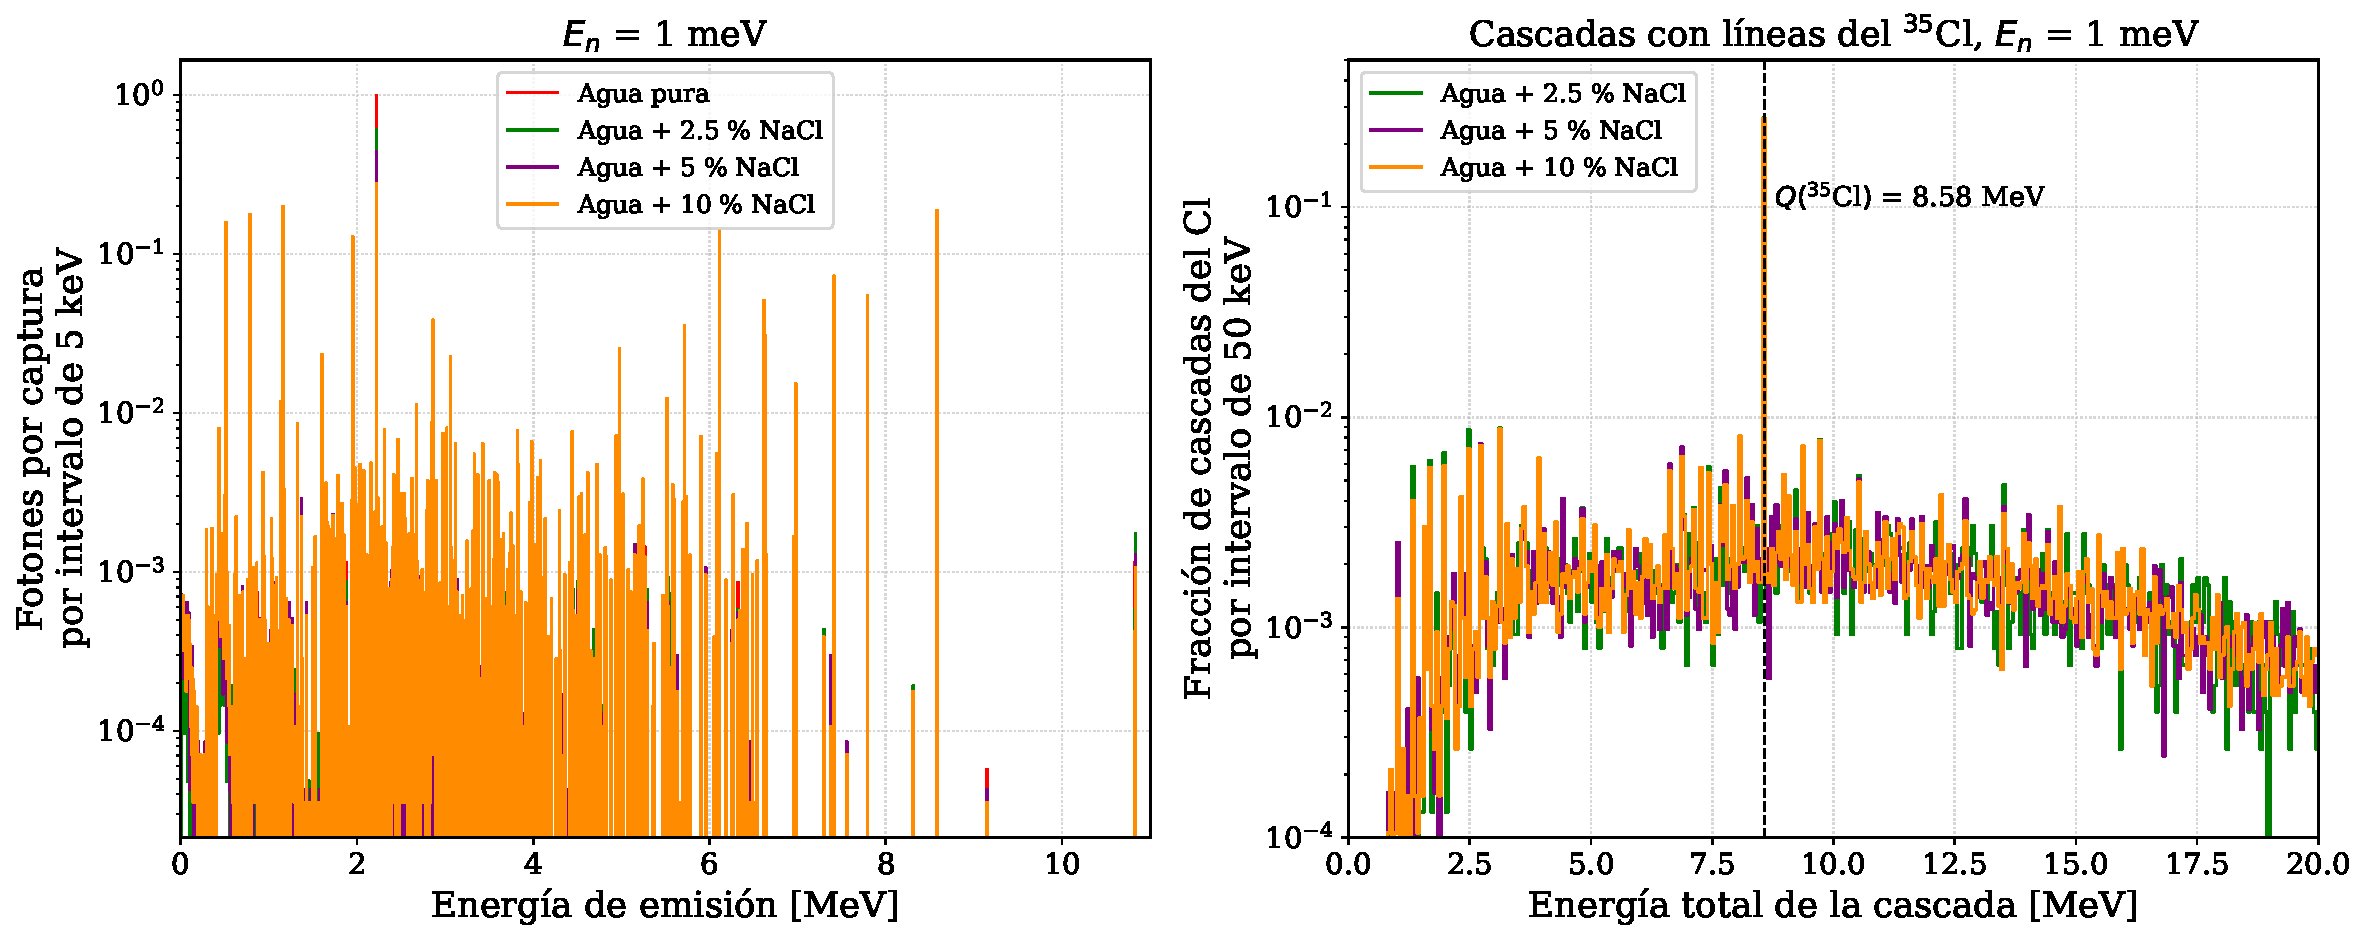
\includegraphics[width=\linewidth]{fig_nueva_emision_y_cascadas.pdf}
  \caption{Izquierda: espectro exacto de emisión de los fotones de captura por captura, a 1~meV. Derecha: energía total de las cascadas que contienen líneas del $^{35}$Cl; la línea discontinua es el valor $Q$ = 8.58~MeV.}
  \label{fig:cascadas}
\end{figure}

El espectro de emisión (Figura~\ref{fig:cascadas}, izquierda) contiene las líneas esperadas: 2.2244~MeV del H en todos los medios y, con NaCl, las líneas del $^{35}$Cl (8.578, 7.790, 7.414, 6.628, 6.620, 6.111, 5.715, 1.959, 1.951, 1.165, 0.788, 0.786 y 0.517~MeV, entre otras) y del $^{23}$Na. Las posiciones de las líneas no dependen de la energía del neutrón, como exige la física de la captura.

Sin embargo, la energía total de las cascadas del Cl no es la energía de separación del neutrón en el $^{36}$Cl ($Q$ = 8.5794~MeV). Solo el 26--27~\% de ellas suma $Q$ dentro de $\pm0.05$~MeV; el resto se distribuye en un continuo ancho, con cascadas de 1~MeV hasta más de 40~MeV, y la energía media es 10.1--10.3~MeV (Figura~\ref{fig:cascadas}, derecha; Tabla~\ref{tab:cascadas}), un 18--20~\% más que $Q$. El resultado es el mismo en las cinco energías y las tres concentraciones. En cambio, las capturas en H emiten siempre un único fotón de 2.2244~MeV, y las del $^{14}$N, uno de 10.83~MeV.

Este comportamiento es compatible con el modelo de emisión no correlacionada del estado final de captura de \texttt{G4NeutronHP}, que muestrea la multiplicidad y la energía de cada fotón a partir de las distribuciones evaluadas sin imponer que la cascada sume $Q$. Para un núcleo con un único fotón (H, $^{14}$N) no hay diferencia, pero para el $^{35}$Cl, de esquema de desexcitación rico, la energía por captura deja de conservarse caso por caso, aunque el espectro de líneas sea correcto en promedio por fotón.

\textbf{Impacto.} Si las cascadas del Cl conservaran la energía, la energía gamma emitida por captura a 1~meV sería 4.73, 5.74 y 6.76~MeV con 2.5, 5 y 10~\% de NaCl; la simulación emite 5.30, 6.61 y 7.91~MeV, un 12, 15 y 17~\% más (a 10~meV, un 13, 15 y 16~\% más). Esta sobreestimación se propaga a la energía depositada, a los electrones secundarios, a la luz Cherenkov y a la carga de los medios con NaCl, y no afecta al agua pura. No modifica los resultados neutrónicos (captura, reflexión, $\lambda_\mathrm{cap}$), que no dependen de la emisión gamma.

\textbf{Recomendación.} Verificarlo con una corrida corta del simulador (por ejemplo, 1~meV con 10~\% de NaCl) activando la emisión de fotones de captura que conserva la energía (en \textsc{Geant4}~11, mediante las opciones de \texttt{G4ParticleHPManager} o las variables de entorno de \texttt{G4NEUTRONHP} que fuerzan la desexcitación con \texttt{G4PhotonEvaporation}), y comparar la energía de las cascadas, la carga media y la eficiencia de detección con las de este informe. Hasta entonces, las cifras de carga y fotoelectrones de los medios con NaCl deben interpretarse como un límite superior.

% =====================================================================
\section{Interacciones y destino de los fotones}
\label{sec:interacciones}

\subsection{Interacciones en el tanque}

\begin{table}[H]
\centering\footnotesize
\caption{Fotones e interacciones con definiciones homogéneas: capturas, trazas de fotones del neutrón y secundarias, pasos totales, pasos en el tanque, dispersiones Compton y fotoabsorciones en el tanque, y pasos fuera del tanque. Compárese con la Tabla~4.10 de la tesis (Sección~\ref{sec:verificacion}).}
\label{tab:interacciones}
\setlength{\tabcolsep}{3.2pt}
\begin{tabular}{@{}lrrrrrrrr@{}}
\toprule
Medio & $N_\mathrm{Cap}$ & $\gamma$ del n & $\gamma$ secund. & Pasos & Tanque & Compton & Fotoabs. & Exterior \\
\csname @@input\endcsname \tablas/tabla_interacciones.tex
\bottomrule
\end{tabular}
\end{table}

\begin{table}[H]
\centering\footnotesize
\caption{Intervalo (sobre las dieciséis energías) de los fotones por captura, del reparto de las interacciones físicas en el tanque (\%), de la fracción de fotones absorbidos en el tanque (\%) y de las dispersiones Compton y fotoabsorciones en el tanque por captura.}
\label{tab:fracciones}
\setlength{\tabcolsep}{2.6pt}
\begin{tabular}{@{}lrrrrrrrrr@{}}
\toprule
& \multicolumn{2}{c}{$\gamma$/captura} & \multicolumn{4}{c}{Interacciones físicas en el tanque [\%]} & Absorbidos & \multicolumn{2}{c}{Por captura} \\
\cmidrule(lr){2-3}\cmidrule(lr){4-7}\cmidrule(lr){9-10}
Medio & del n & secund. & Compton & Fotoel. & Rayleigh & Pares & [\%] & Compton & Fotoel. \\
\midrule
\csname @@input\endcsname \tablas/tabla_fracciones.tex
\bottomrule
\end{tabular}
\end{table}

La dispersión Compton es el 88--90~\% de las interacciones físicas en el tanque, en todos los medios y energías, seguida por la absorción fotoeléctrica (5.8--8.1~\%), la dispersión Rayleigh (3.5--3.9~\%) y la producción de pares (0.12--0.71~\%), como corresponde a fotones de 0.05--10~MeV en un medio de $Z$ bajo. Al añadir NaCl, la fracción Compton baja ligeramente y suben la fotoeléctrica y la de pares, por el mayor número atómico efectivo y por las líneas del Cl por encima del umbral de pares. La fracción Compton de la tesis (0.697--0.756) es menor porque se calcula respecto a todos los pasos en el tanque, incluidos los de \var{Transportation}.

\textbf{La salinidad actúa a través de la fuente.} El número bruto de dispersiones Compton en el tanque a 1~meV es 3.15 veces mayor con 10~\% de NaCl que en agua pura, el ``factor 3'' de la tesis. Ese factor se descompone en $1.61\times2.54\times0.77$: 1.61 veces más capturas, 2.54 veces más fotones por captura (incluidos los secundarios) y un 23~\% menos de dispersiones por fotón (a 1~eV y 1~keV, $1.43\times2.49\times0.78$ y $1.34\times2.49\times0.80$). Por captura, la razón es 1.95 (9.0 frente a 4.6 dispersiones). El número de dispersiones por fotón disminuye porque los fotones más energéticos del Cl escapan con más facilidad: la energía media al escapar es 1.34~MeV en agua pura y 2.28~MeV con 10~\% de NaCl. El aumento de los conteos con la salinidad se debe, por tanto, al término fuente y no a un aumento de las probabilidades de interacción por fotón.

\begin{figure}[H]
  \centering
  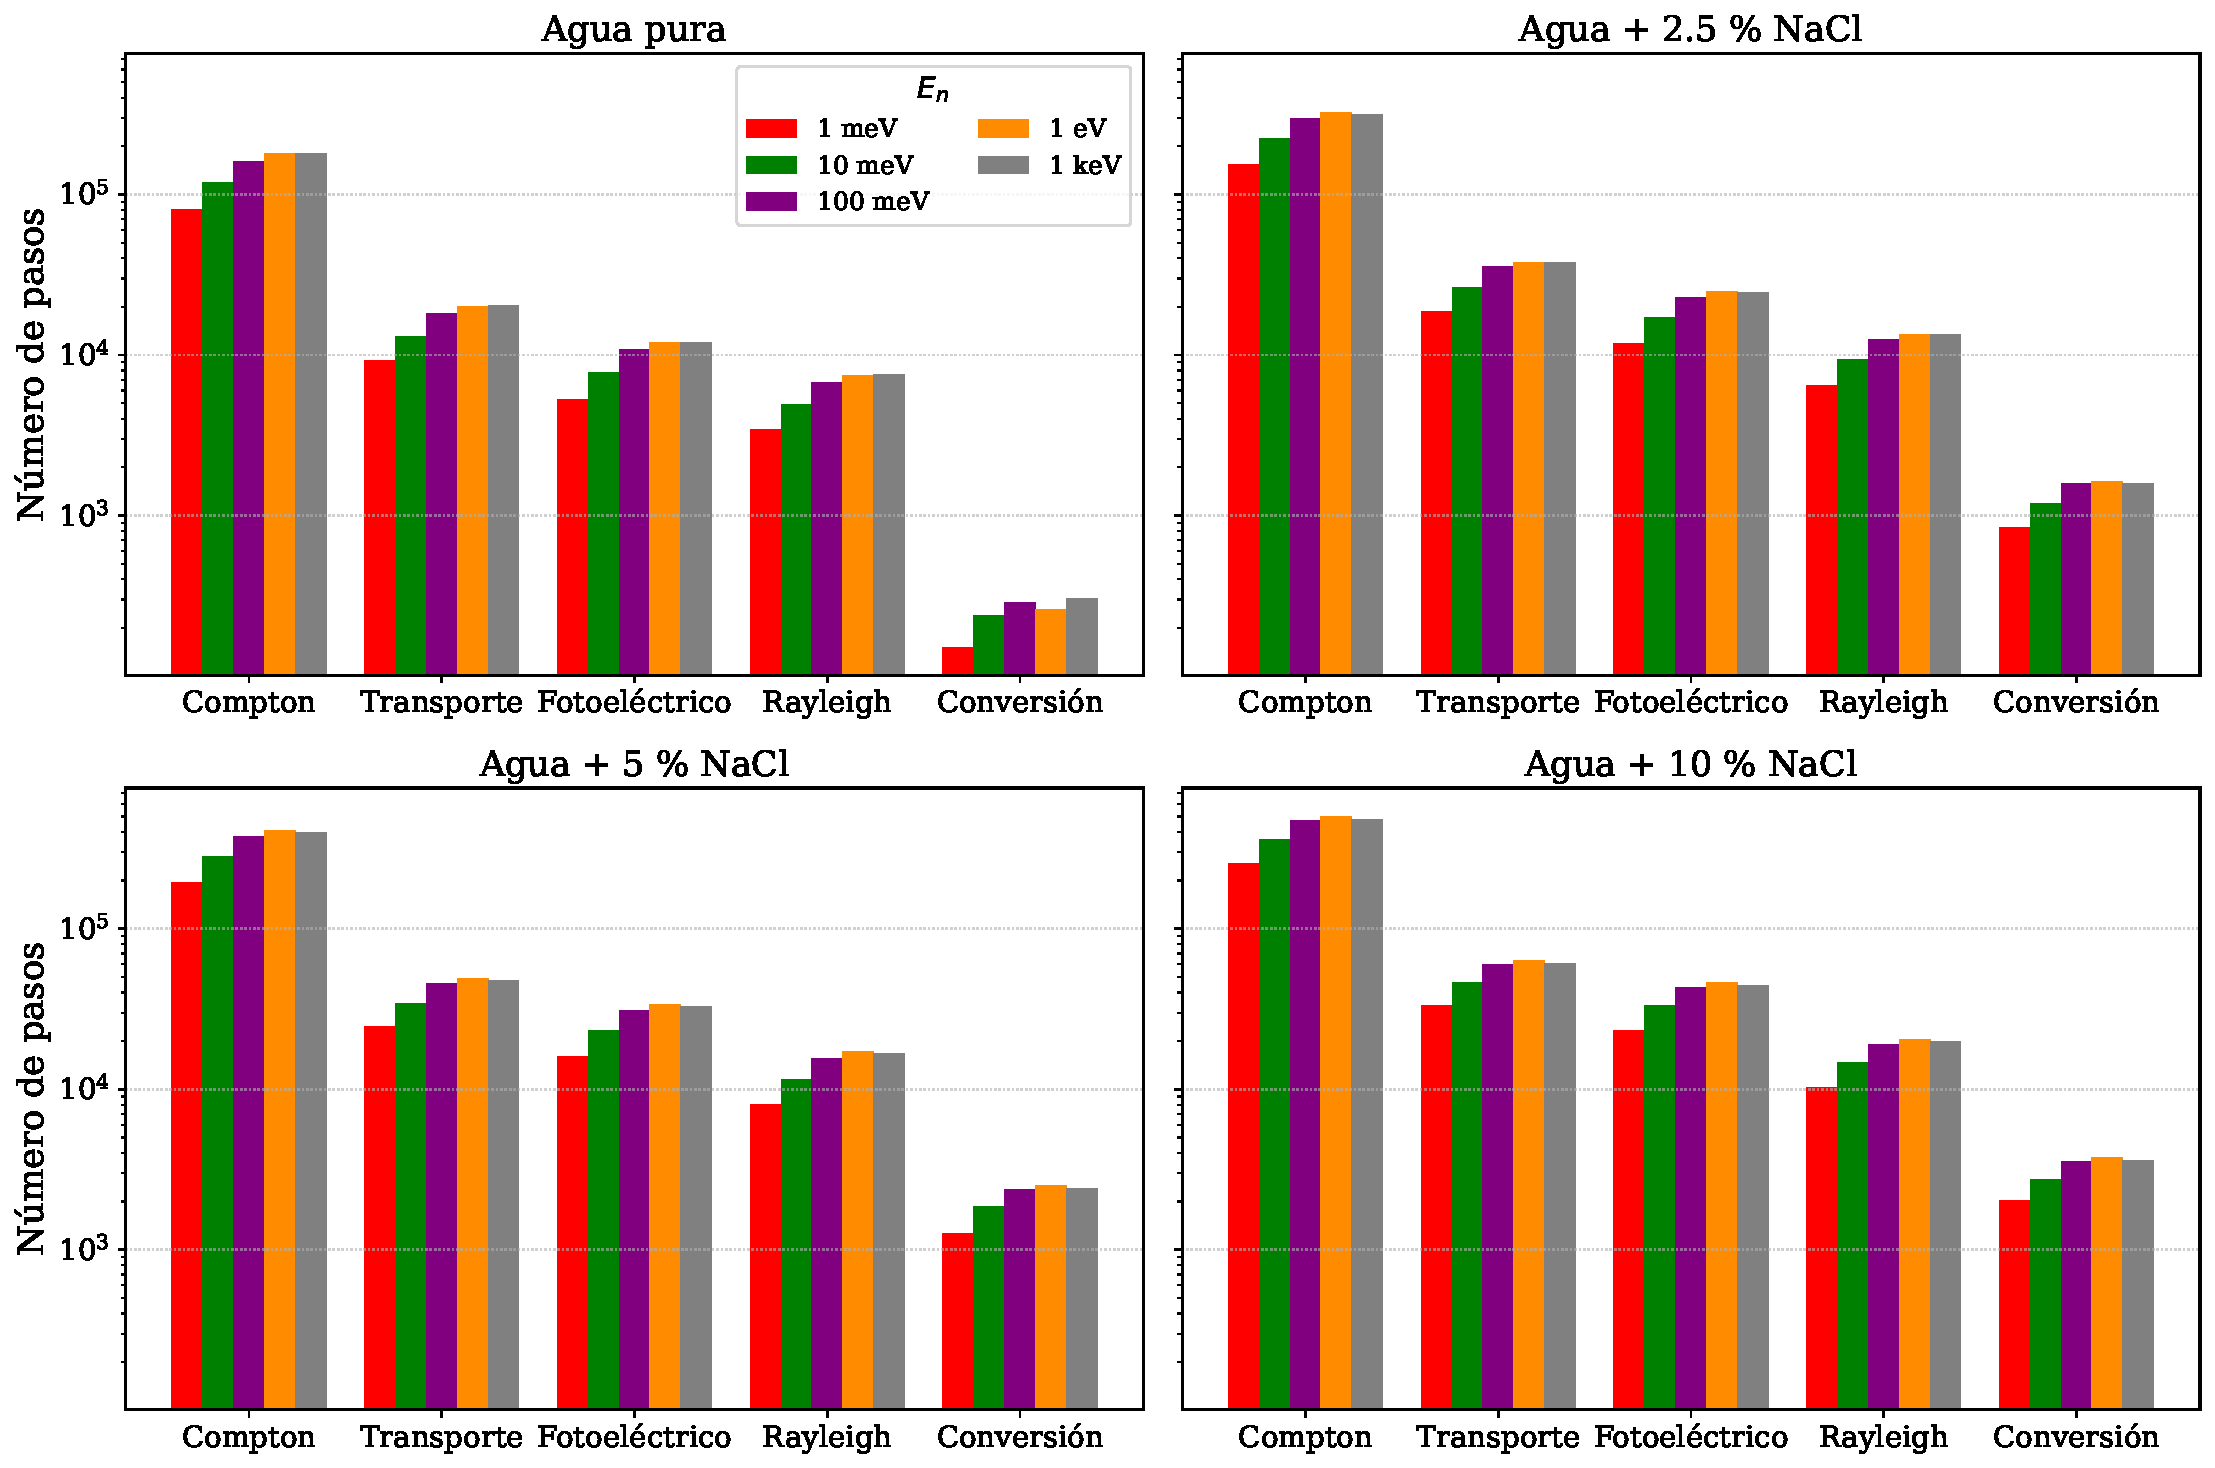
\includegraphics[width=0.95\linewidth]{fig_4_30_procesos_tanque.pdf}
  \caption{Pasos por proceso en el tanque estricto para cinco energías y los cuatro medios (Figura~4.30 de la tesis).}
  \label{fig:procesos}
\end{figure}

\begin{figure}[H]
  \centering
  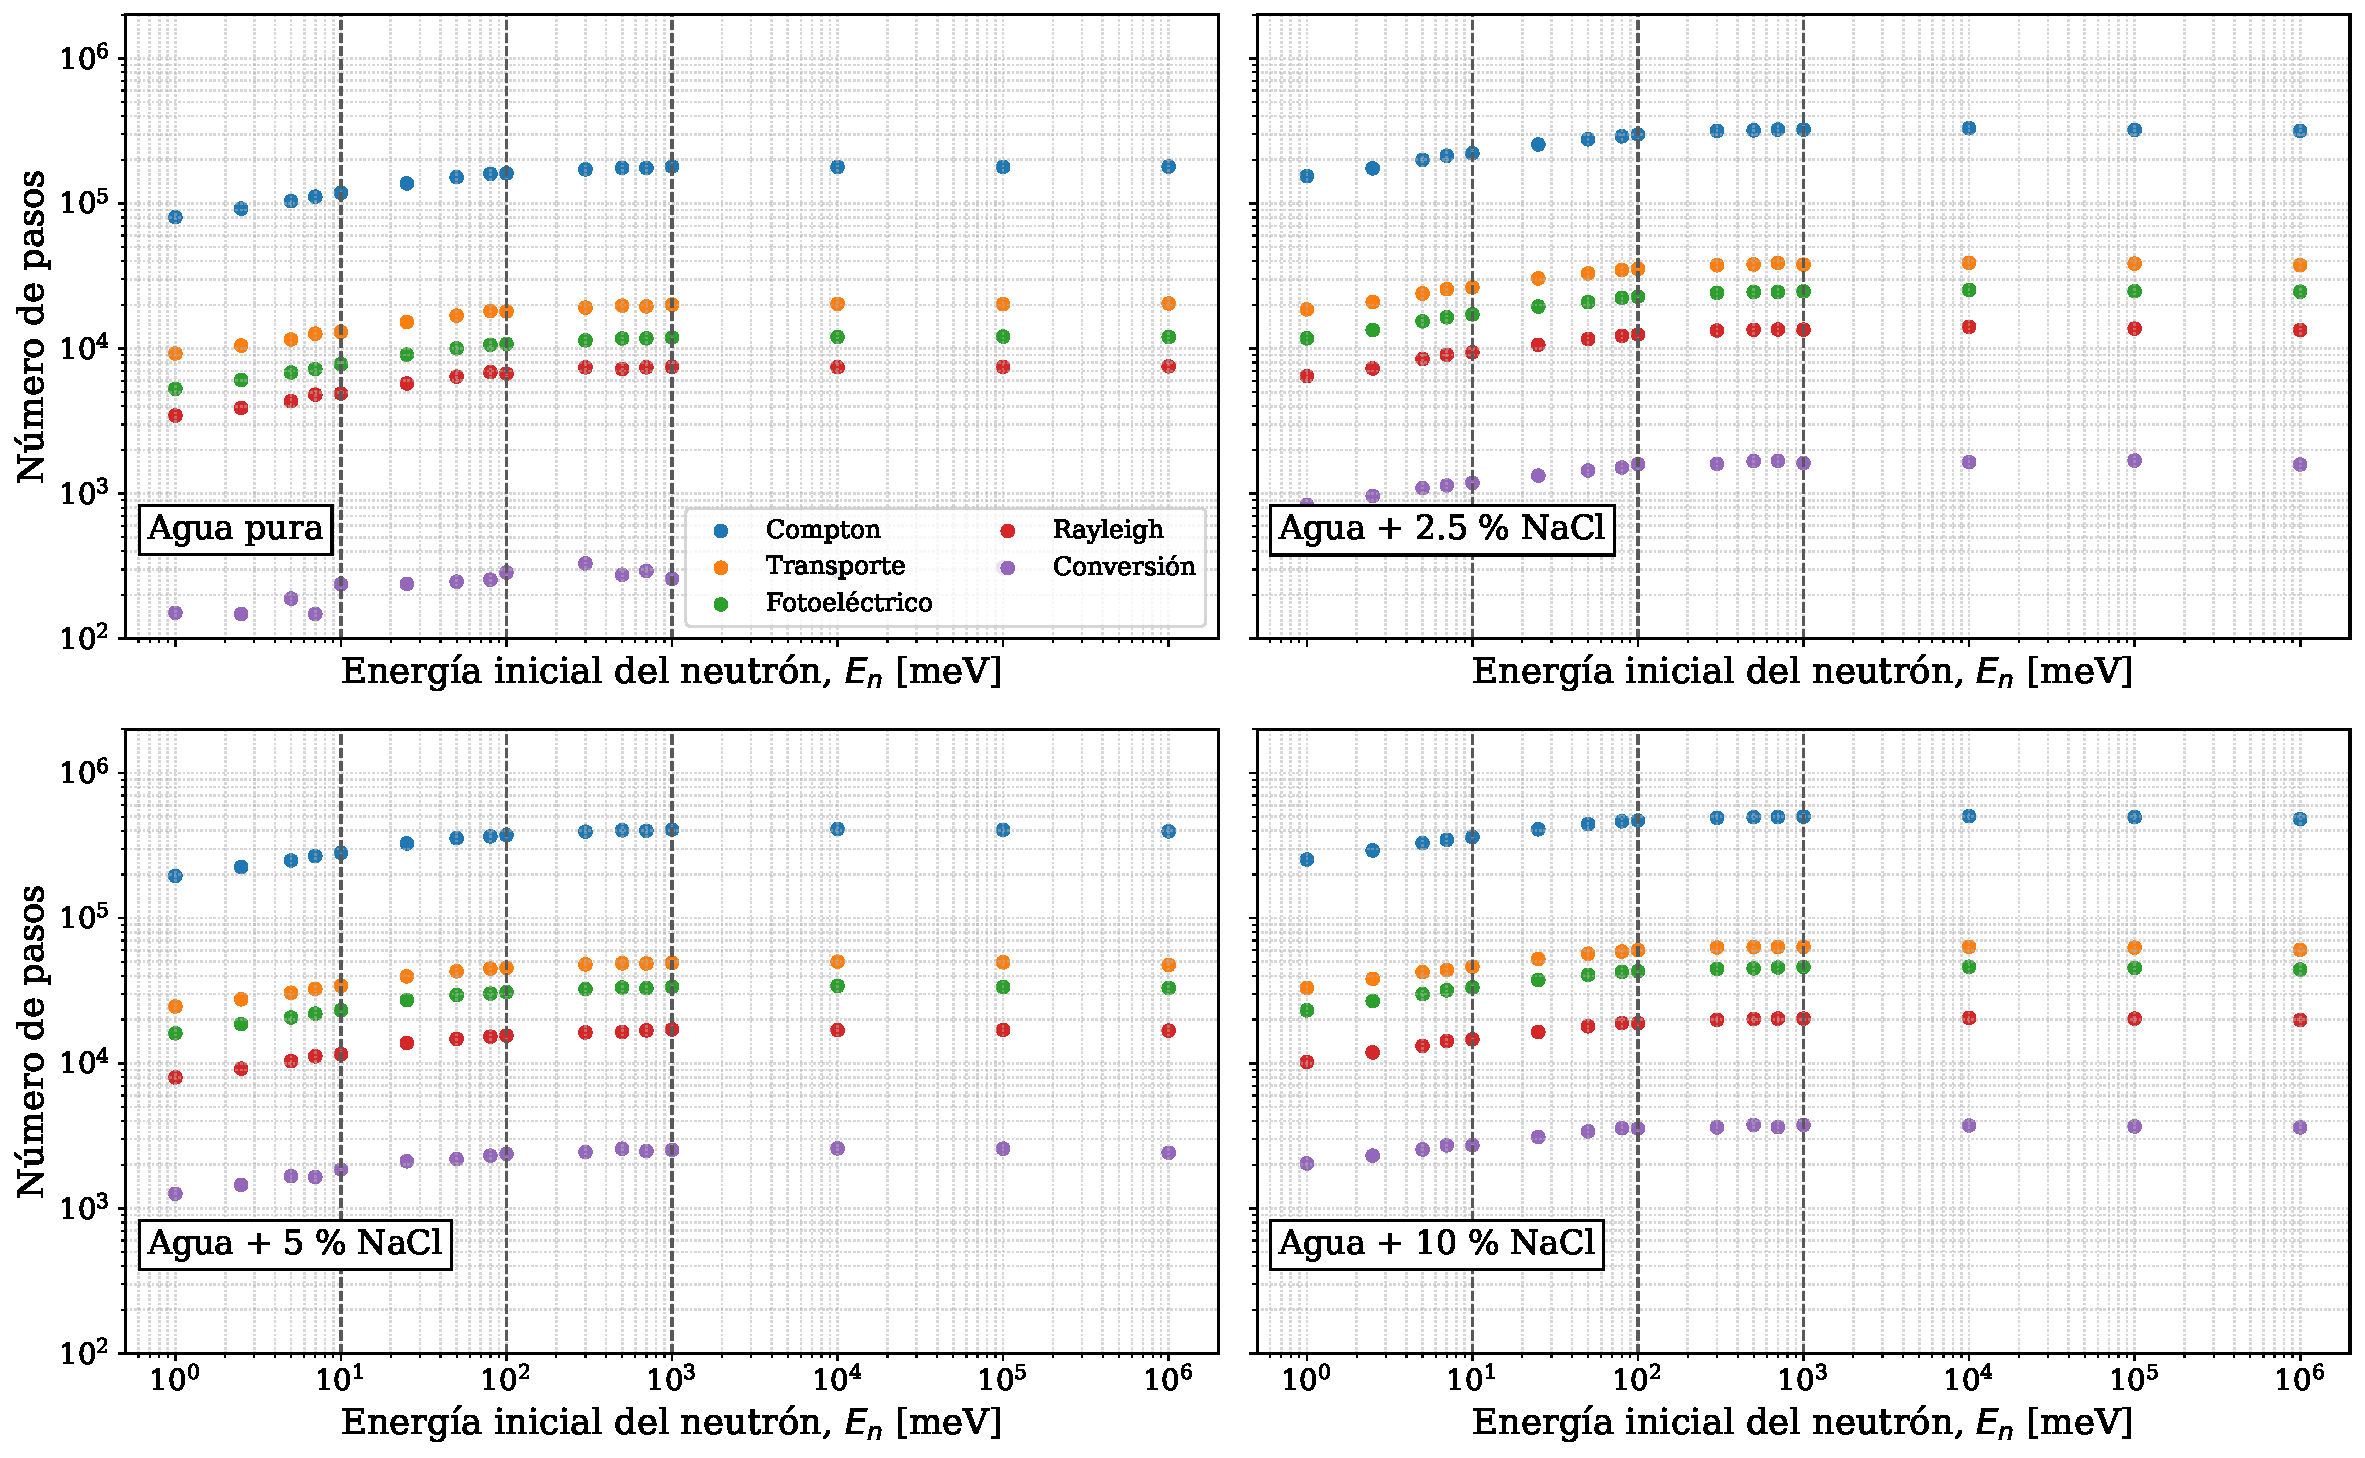
\includegraphics[width=0.95\linewidth]{fig_4_32_procesos_vs_energia.pdf}
  \caption{Pasos por proceso en el tanque estricto frente a la energía del neutrón (Figura~4.32 de la tesis, corregida: los valores se leen de los resúmenes en lugar de transcribirse).}
  \label{fig:procesos-e}
\end{figure}

\begin{figure}[H]
  \centering
  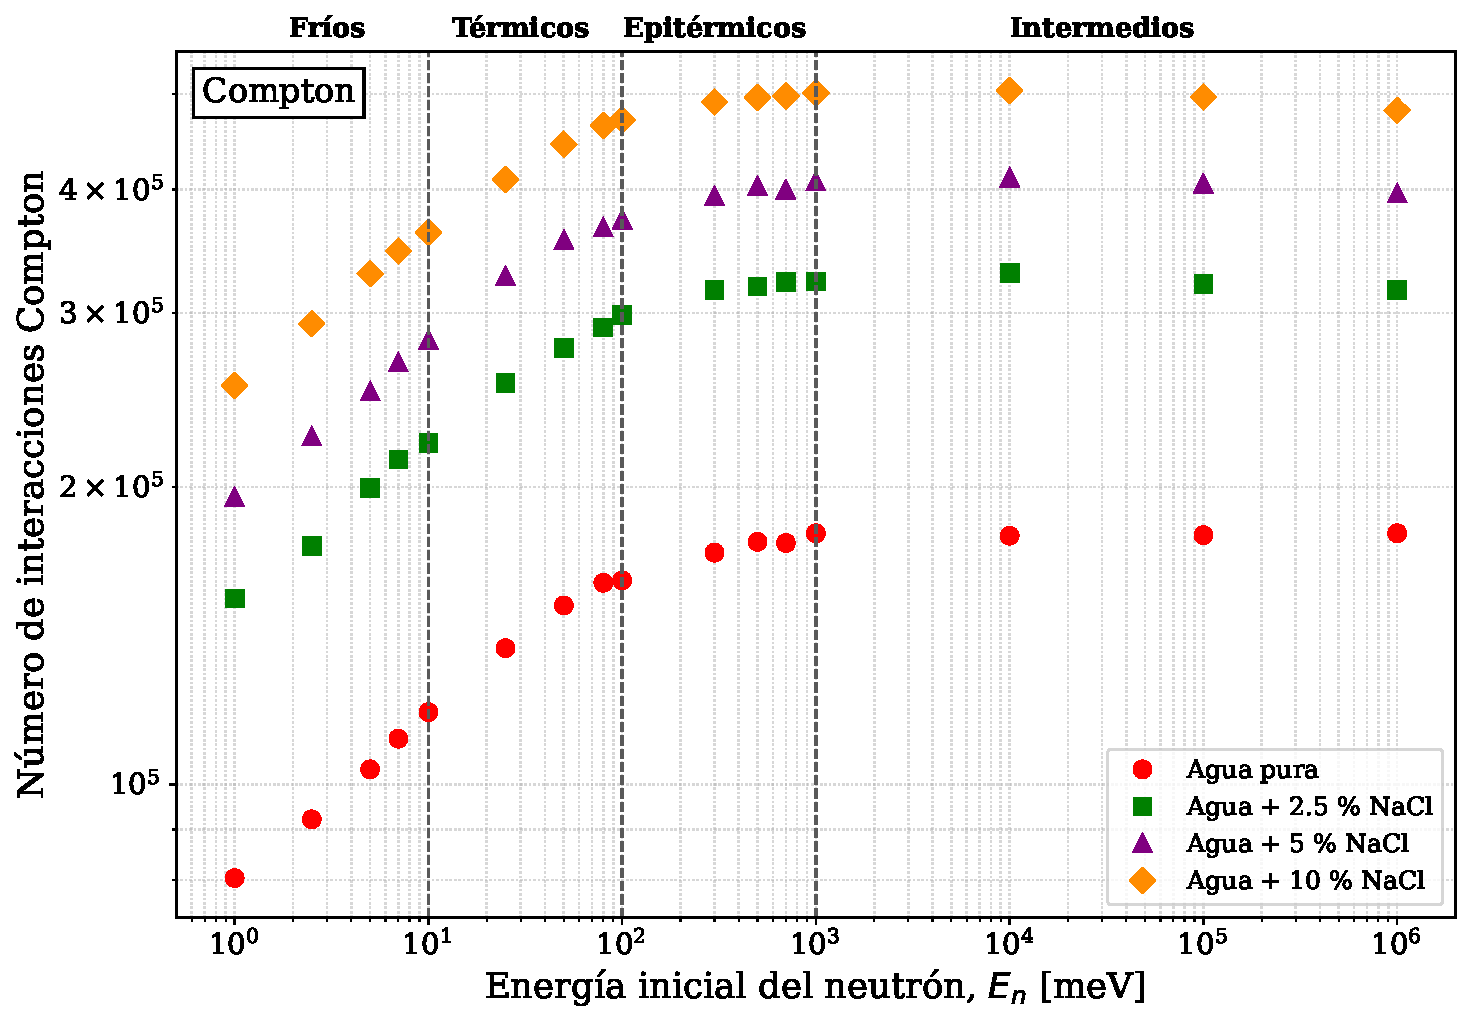
\includegraphics[width=0.49\linewidth]{fig_4_35_compton_vs_energia.pdf}\hfill
  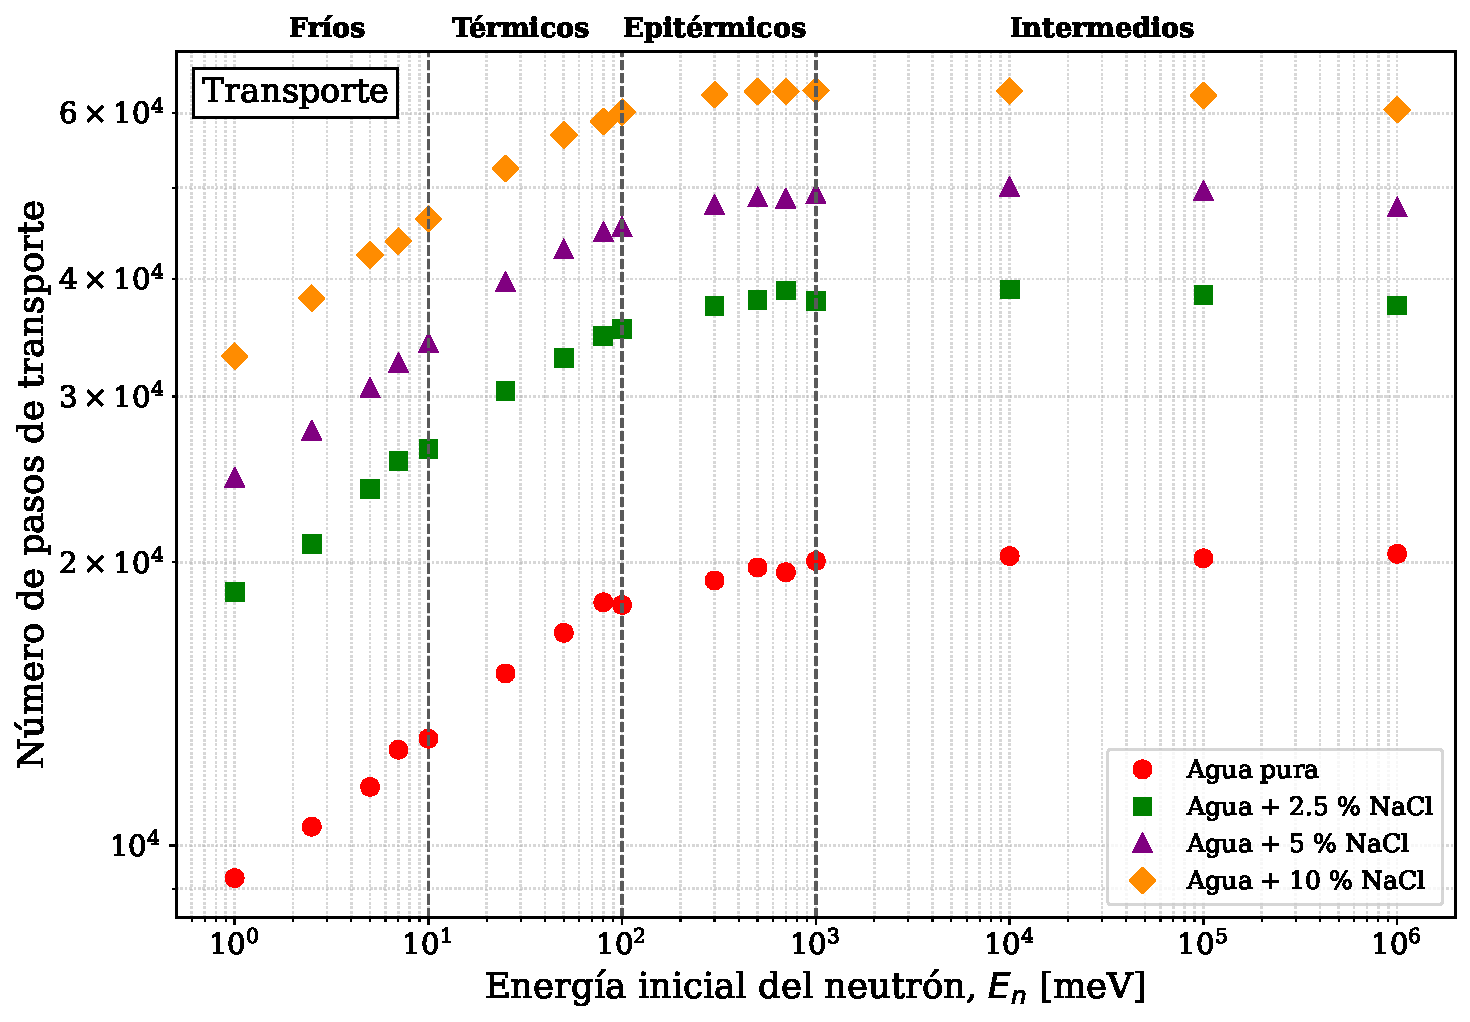
\includegraphics[width=0.49\linewidth]{fig_4_31_transporte_vs_energia.pdf}\\[0.3em]
  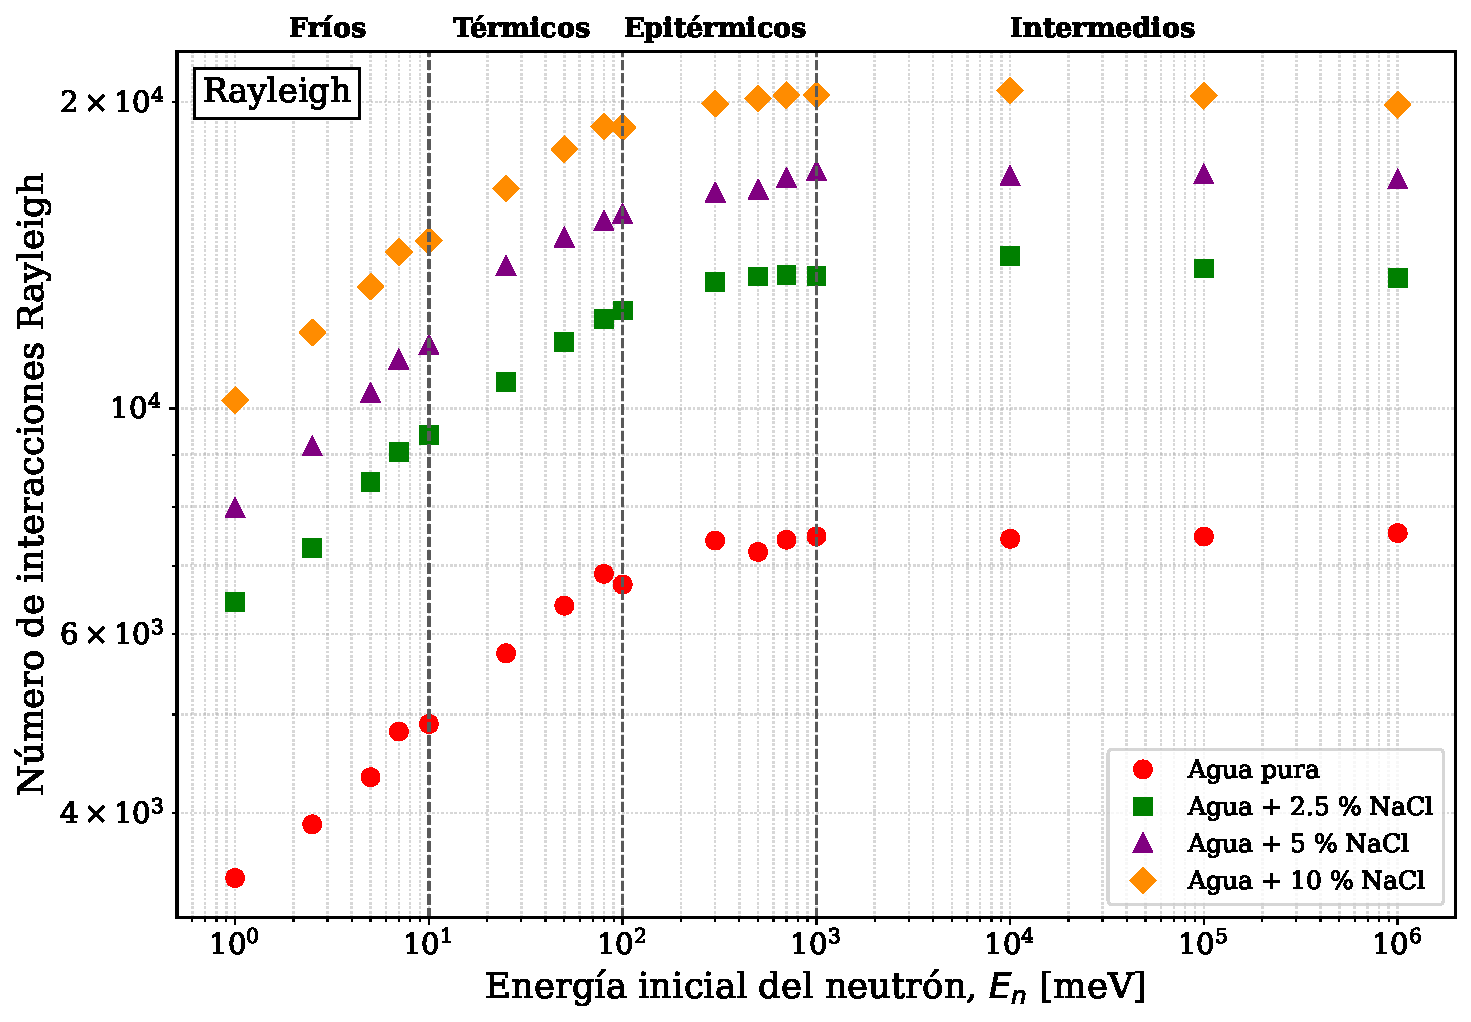
\includegraphics[width=0.49\linewidth]{fig_4_37_rayleigh_vs_energia.pdf}\hfill
  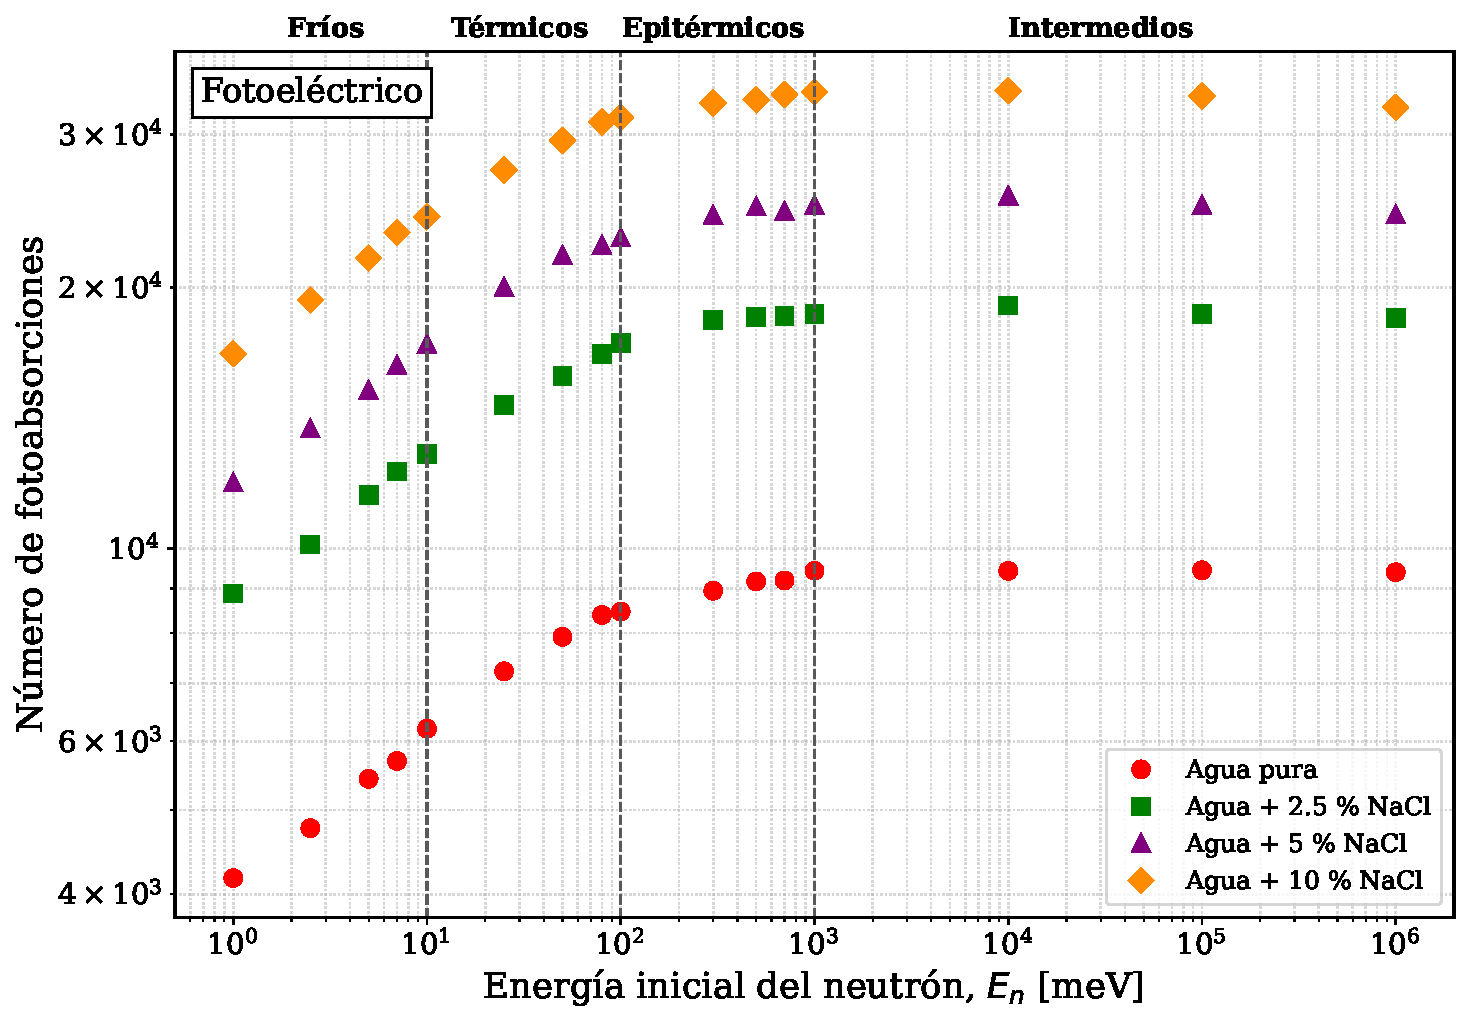
\includegraphics[width=0.49\linewidth]{fig_4_40_fotoelectrico_vs_energia.pdf}
  \caption{Dispersiones Compton, pasos de transporte, dispersiones Rayleigh y fotoabsorciones frente a la energía del neutrón (Figuras~4.35, 4.31, 4.37 y 4.40 de la tesis, corregidas). Las fotoabsorciones siguen la definición de la tesis (paso \var{phot} precedido de \var{compt} en el tanque estricto).}
  \label{fig:vs-e}
\end{figure}

Todos los conteos siguen la forma de la captura: crecen desde el régimen frío, tienen una meseta entre 300~meV y 10~eV y bajan ligeramente hacia 1~keV. Esa forma es la del término fuente, no la de una dependencia de las secciones eficaces gamma con la energía del neutrón.

\subsection{Destino de los fotones}

\begin{figure}[H]
  \centering
  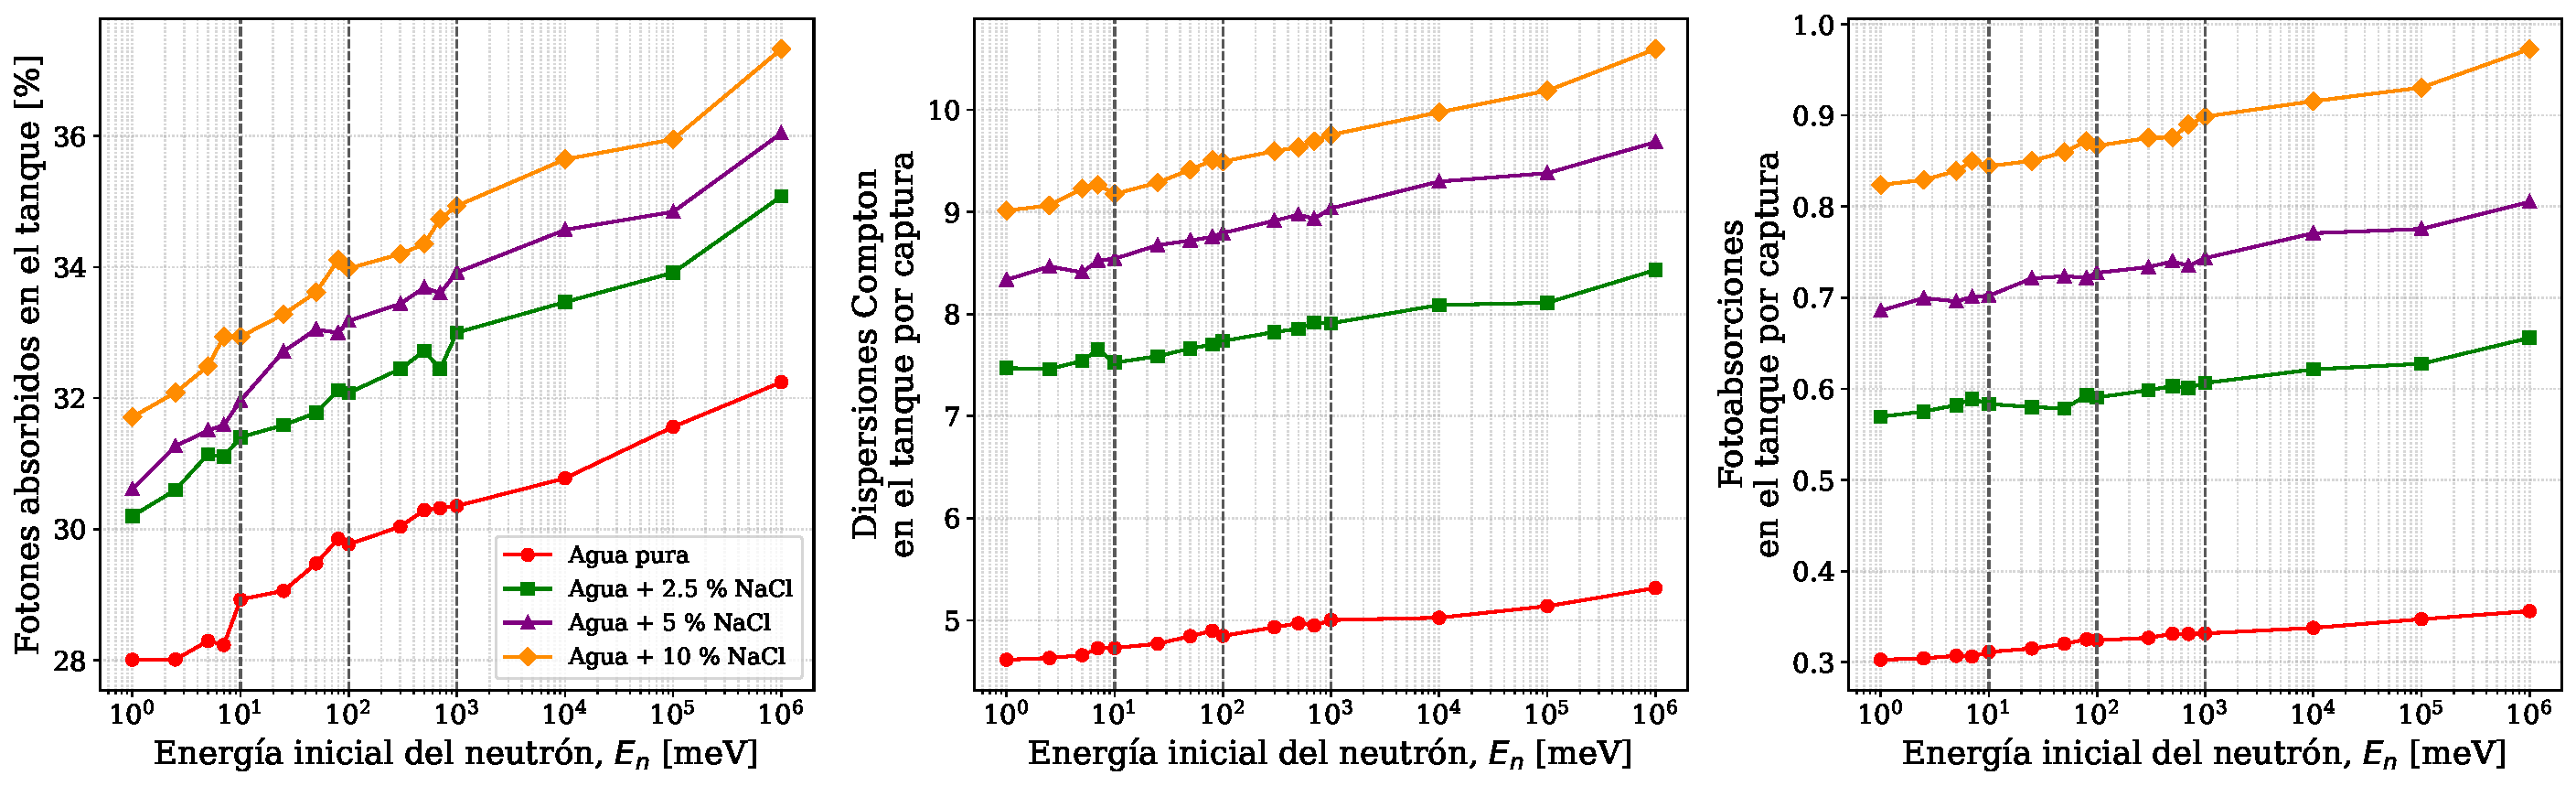
\includegraphics[width=\linewidth]{fig_nueva_destino_y_rendimiento.pdf}
  \caption{Fracción de fotones absorbidos en el tanque, y dispersiones Compton y fotoabsorciones en el tanque por captura, frente a la energía del neutrón.}
  \label{fig:destino}
\end{figure}

De los 5\,074\,206 fotones de las 64 corridas, solo un 28--37~\% se absorbe en el agua por efecto fotoeléctrico o producción de pares; el resto escapa del tanque, casi siempre después de una o varias dispersiones Compton (Figura~\ref{fig:destino}). La fracción absorbida aumenta con la salinidad (de 28--32~\% en agua pura a 32--37~\% con 10~\% de NaCl) y con la energía del neutrón, lo que es compatible con capturas algo más profundas (la longitud de captura crece con la energía), cuyos fotones atraviesan más agua antes de alcanzar la tapa. Un 16--21~\% de los pasos de los fotones ocurre fuera del tanque (tapa, aire, estructura), como indica la tesis.

% =====================================================================
\section{Espectros de energía}
\label{sec:espectros}

\subsection{Energía de los fotones en el tanque}

\begin{figure}[H]
  \centering
  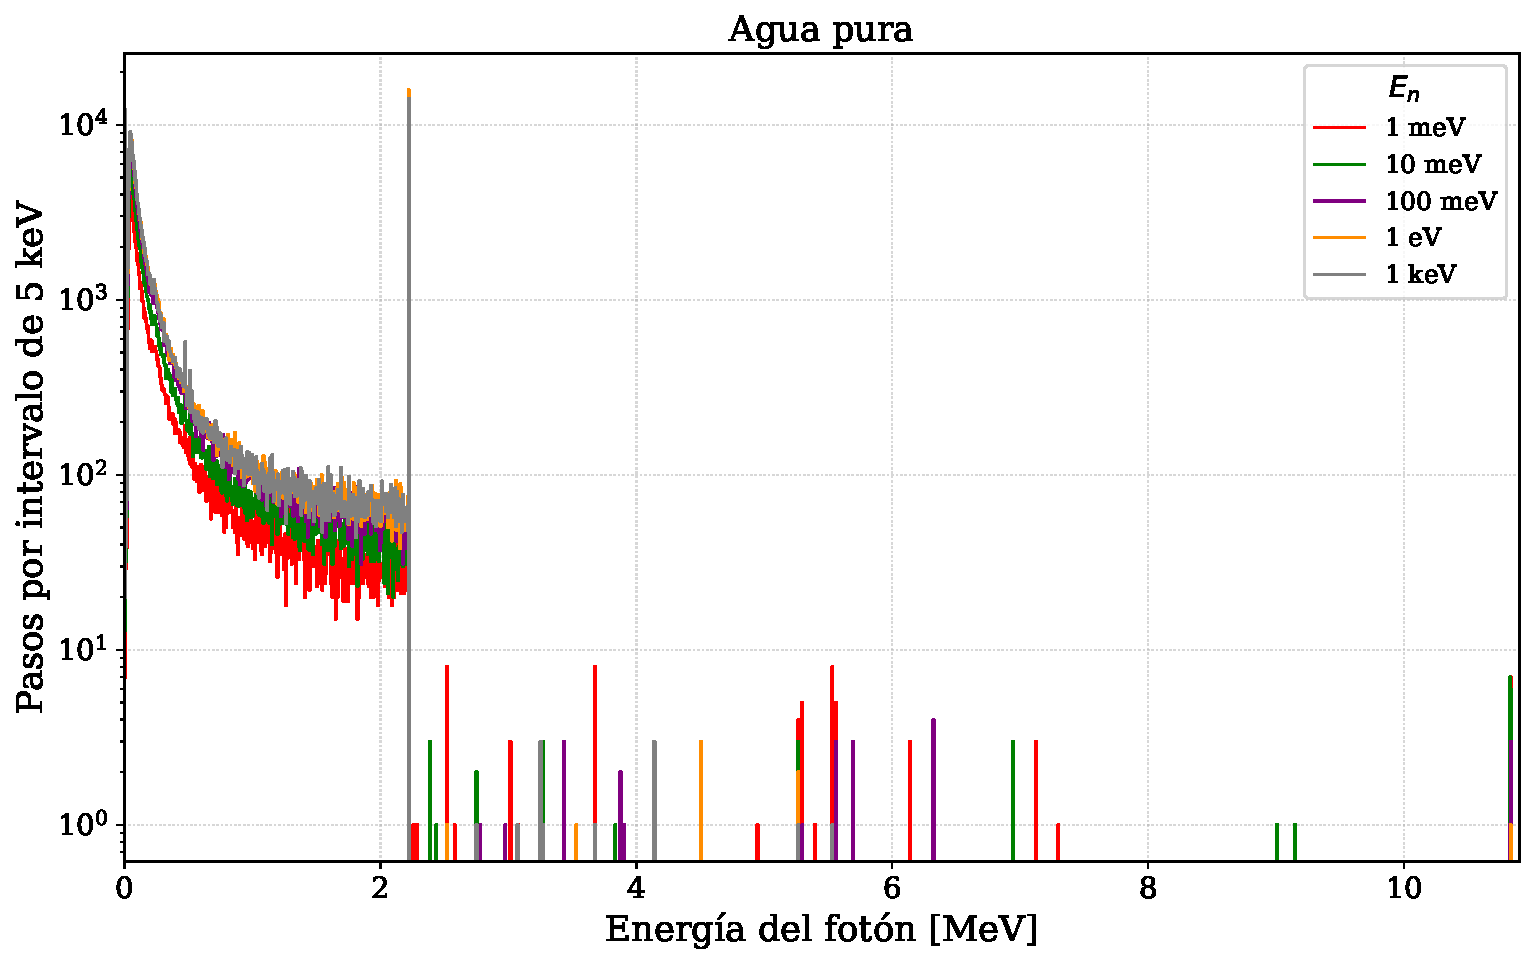
\includegraphics[width=0.49\linewidth]{fig_4_33_espectro_tanque_agua_pura.pdf}\hfill
  \includegraphics[width=0.49\linewidth]{{fig_4_34_espectro_tanque_2.5NaCl}.pdf}
  \caption{Energía de todos los pasos de los fotones en el tanque, en agua pura y con 2.5~\% de NaCl (Figuras~4.33 y 4.34 de la tesis).}
  \label{fig:espectro-tanque}
\end{figure}

En agua pura destaca la línea de 2.224~MeV del H, que corta el continuo Compton: ningún fotón de agua pura supera esa energía, salvo los raros de 10.83~MeV del nitrógeno del aire. Con NaCl, el espectro se extiende hasta 8.6~MeV y aparecen las líneas del Cl y del Na.

\subsection{Dispersión Compton}

\begin{figure}[H]
  \centering
  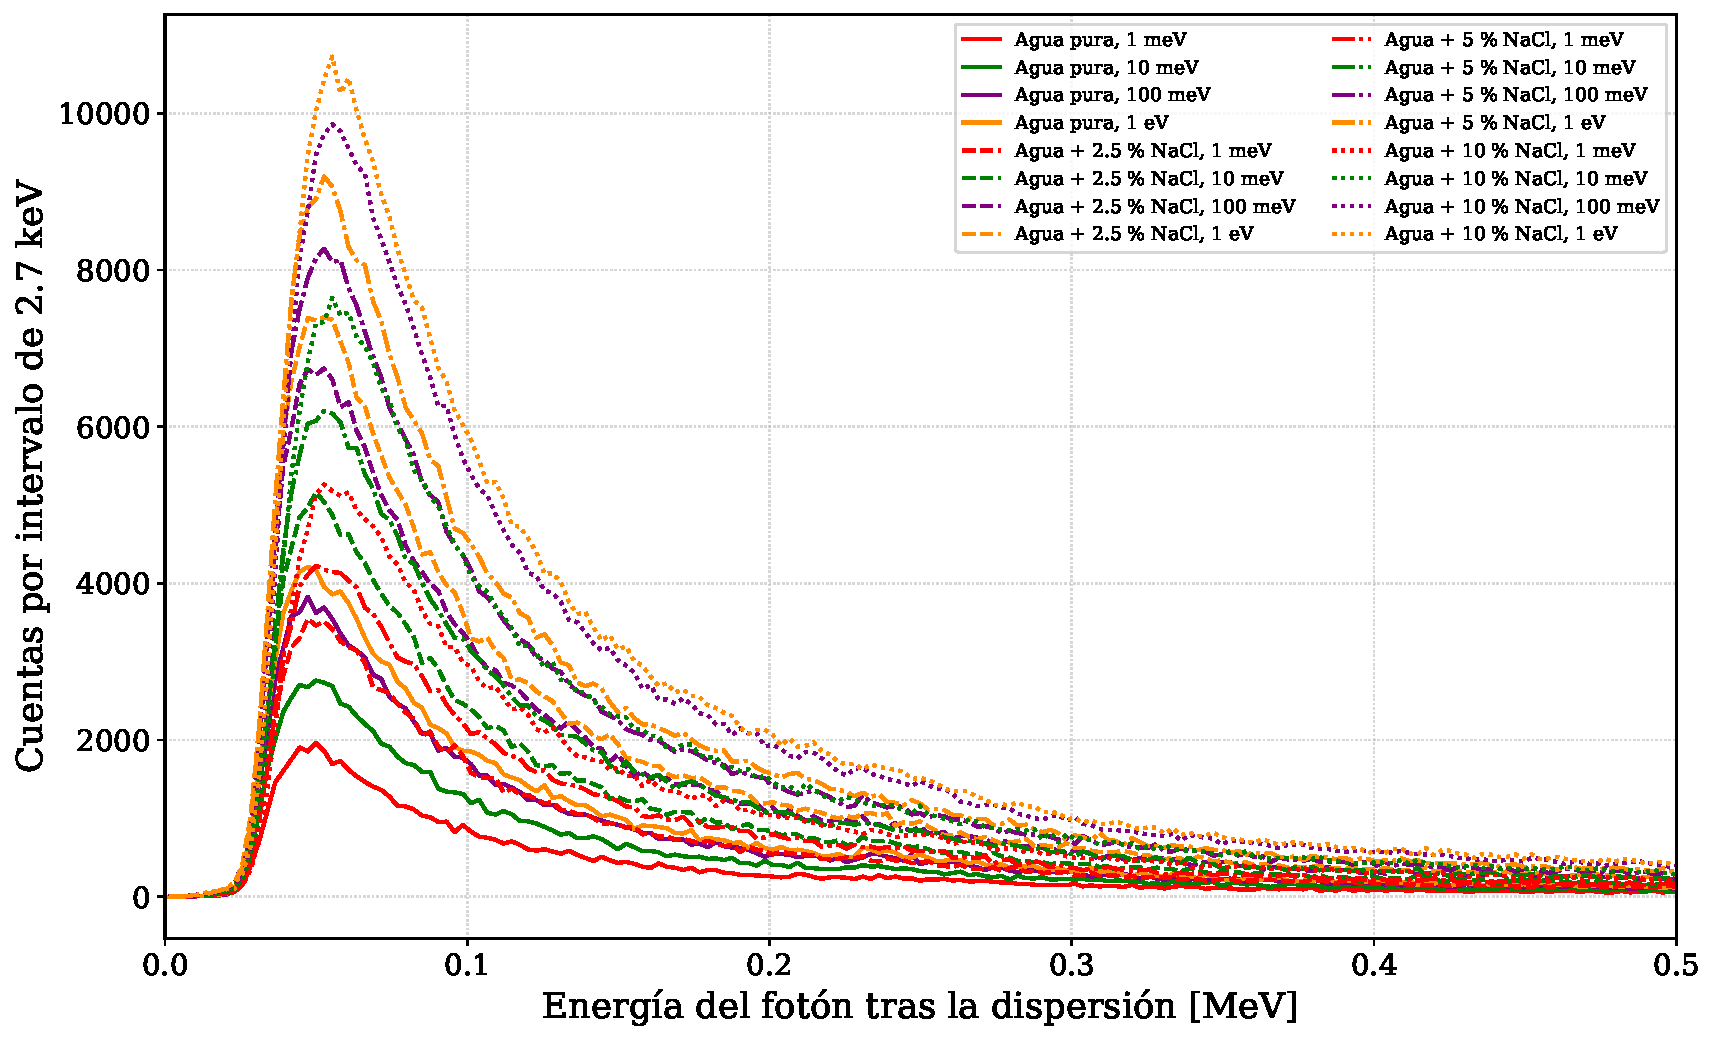
\includegraphics[width=0.85\linewidth]{fig_4_36_espectro_compton.pdf}
  \caption{Energía del fotón tras la dispersión Compton en el tanque estricto (Figura~4.36 de la tesis).}
  \label{fig:compton}
\end{figure}

\begin{table}[H]
\centering\small
\caption{Máximo y FWHM del espectro Compton (1000 intervalos en [0, 2.7]~MeV; tabla de FWHM de la tesis, reproducida).}
\label{tab:fwhm}
\begin{tabular}{@{}llrrr@{}}
\toprule
Medio & $E_n$ & FWHM [MeV] & $E_\mathrm{max}$ [MeV] & $C_\mathrm{max}$ \\
\midrule
\csname @@input\endcsname \tablas/tabla_fwhm.tex
\bottomrule
\end{tabular}
\end{table}

El espectro es un continuo con un máximo entre 0.047 y 0.055~MeV y una cola hacia energías mayores; la FWHM pasa de 0.054--0.057~MeV en agua pura a 0.065--0.070~MeV con 10~\% de NaCl. Este máximo no es una pérdida de energía elemental, sino la acumulación de fotones que, tras varias dispersiones, llegan a decenas de keV, donde la absorción fotoeléctrica termina su historia.

\subsection{Dispersión Rayleigh}

\begin{figure}[H]
  \centering
  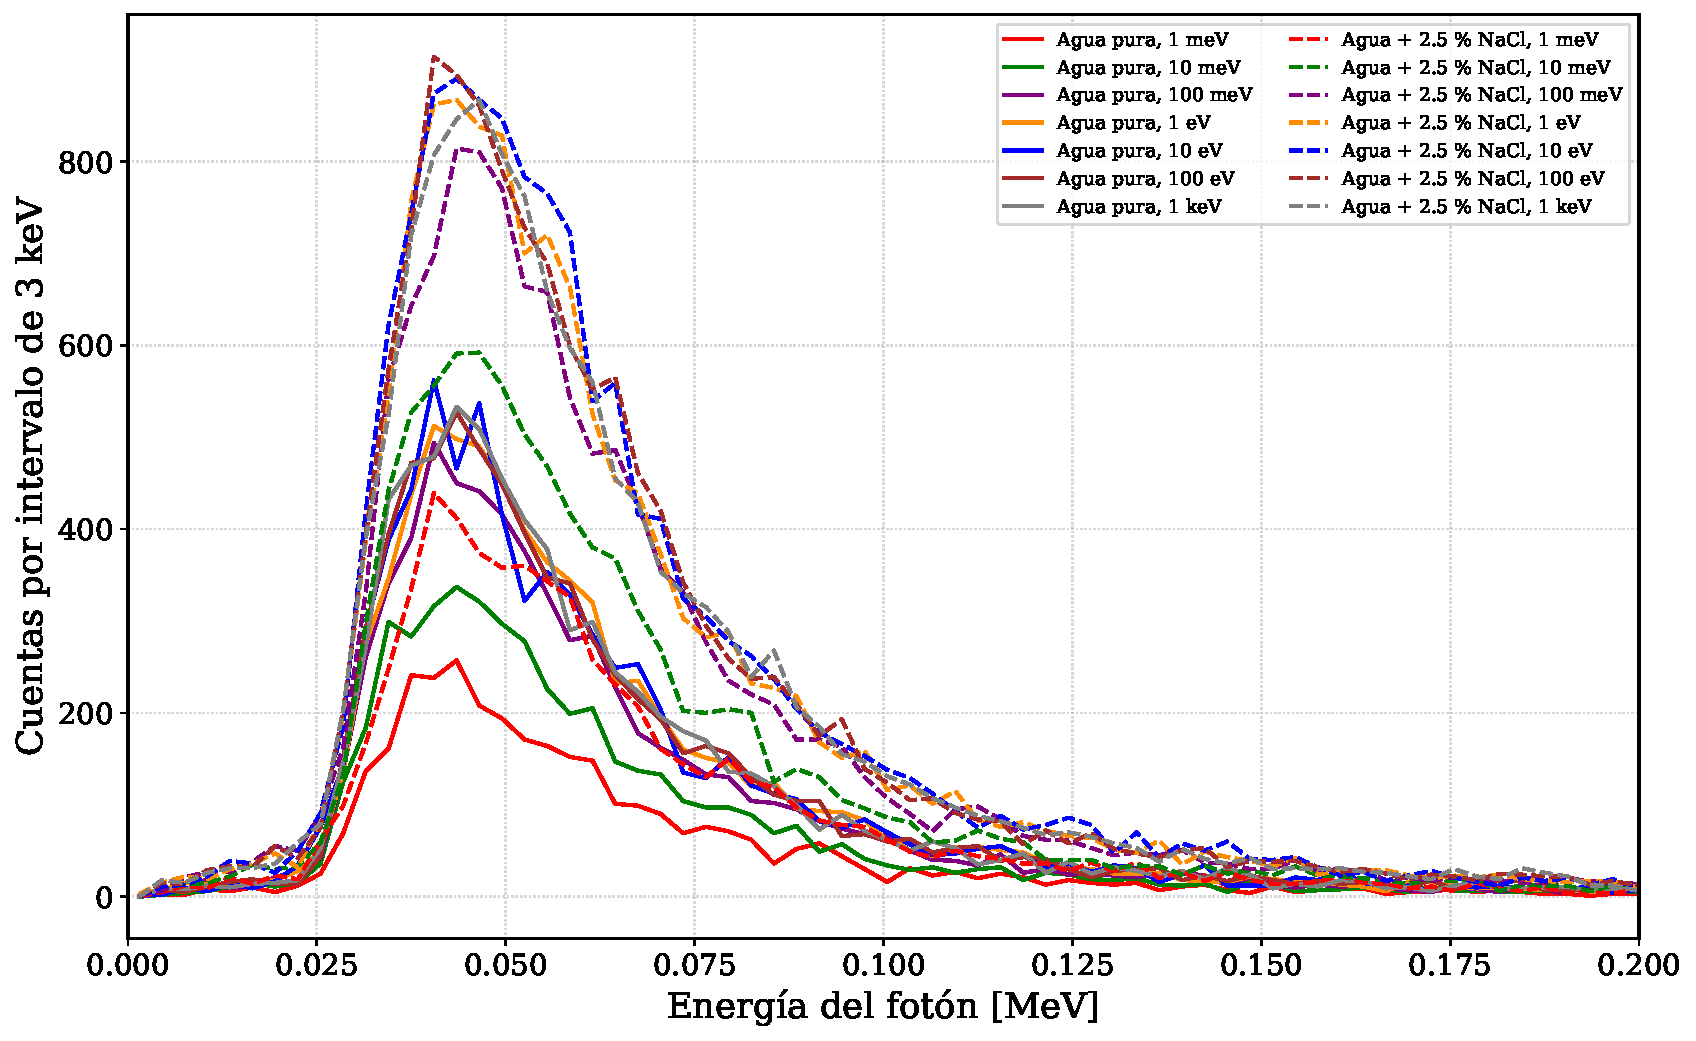
\includegraphics[width=0.85\linewidth]{fig_4_39_espectro_rayleigh.pdf}
  \caption{Energía de los fotones dispersados por Rayleigh en el tanque, en agua pura y con 2.5~\% de NaCl (Figura~4.39 de la tesis).}
  \label{fig:rayleigh}
\end{figure}

La dispersión Rayleigh se concentra por debajo de 0.1~MeV, con un máximo entre 0.0405 y 0.0495~MeV (intervalos de 3~keV), y las líneas de emisión aparecen superpuestas cuando el fotón se dispersa sin haber perdido energía.

\subsection{Absorción fotoeléctrica}

\begin{figure}[H]
  \centering
  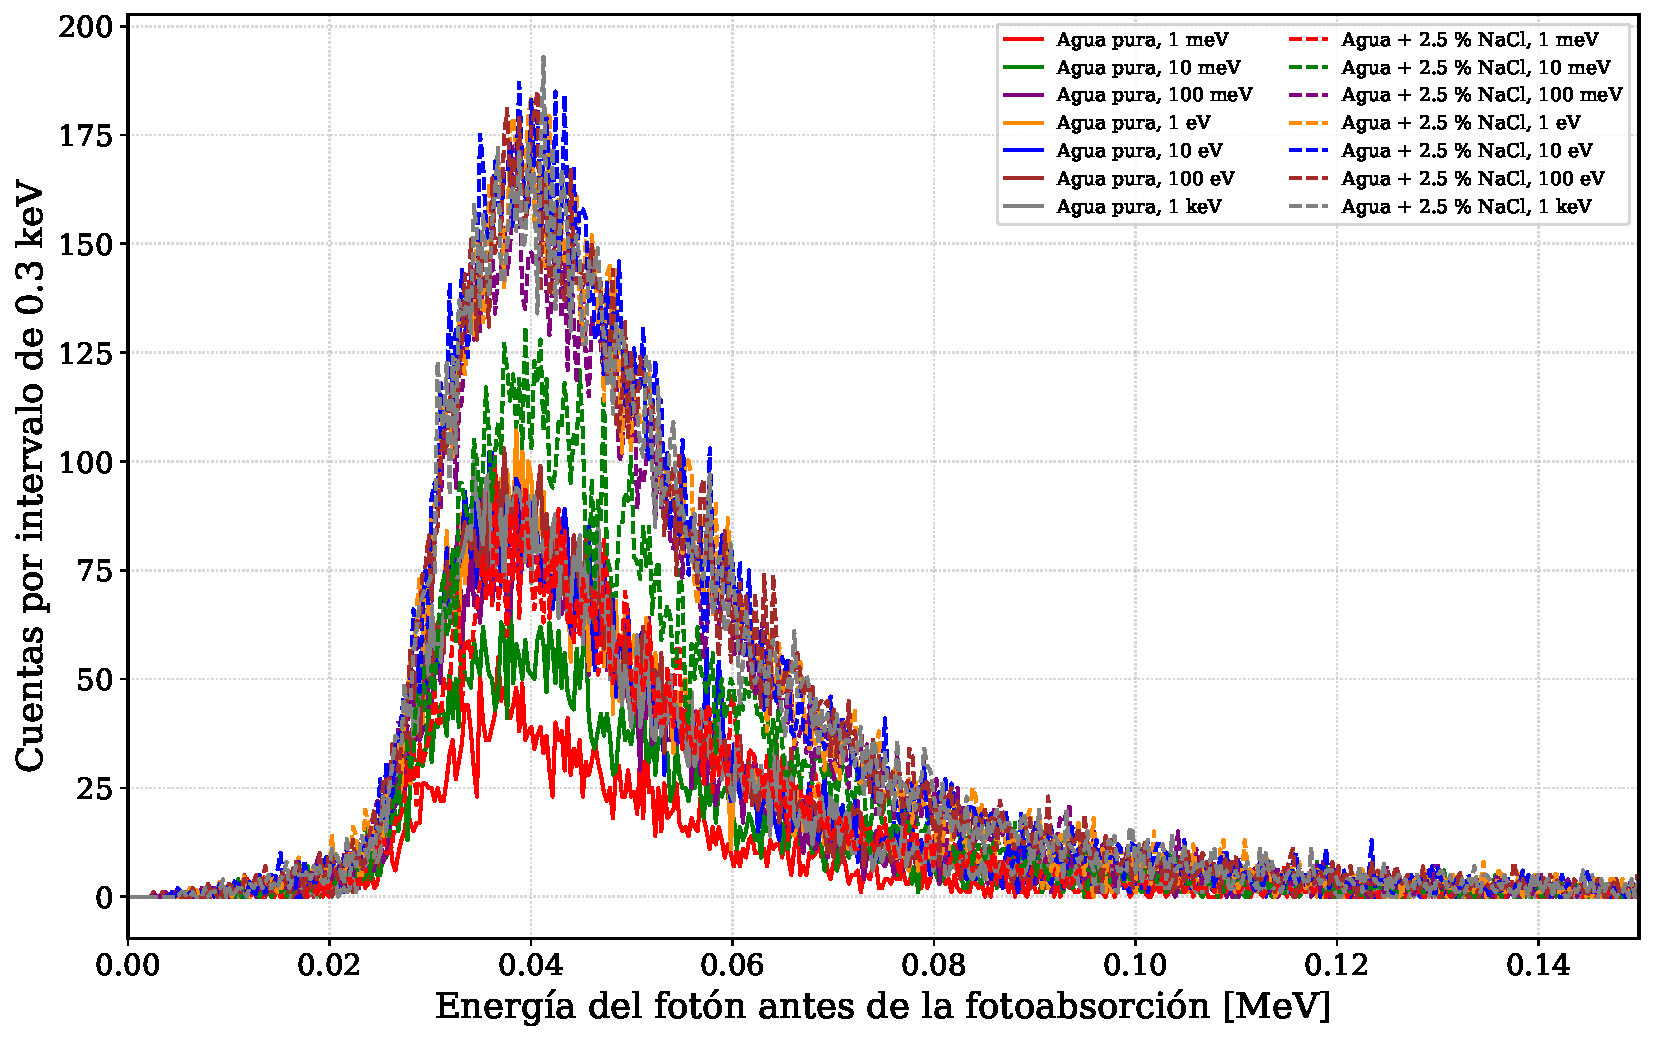
\includegraphics[width=0.85\linewidth]{fig_4_41_espectro_fotoelectrico.pdf}
  \caption{Energía de los fotones antes de la fotoabsorción (definición de la tesis), en agua pura y con 2.5~\% de NaCl (Figura~4.41 de la tesis).}
  \label{fig:fotoel}
\end{figure}

\begin{figure}[H]
  \centering
  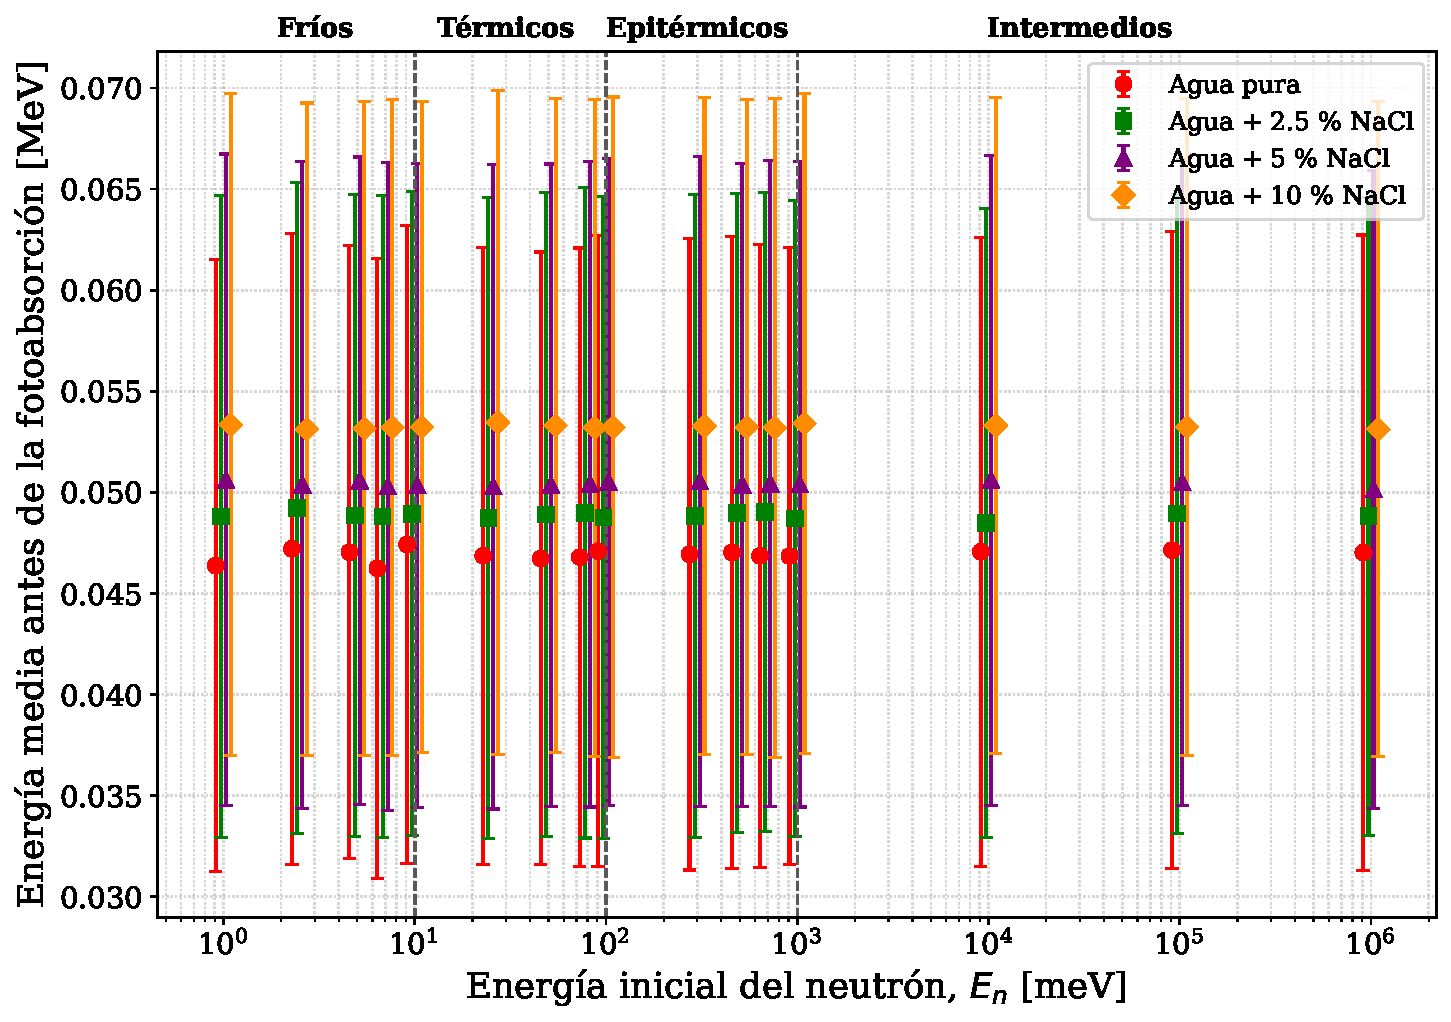
\includegraphics[width=0.75\linewidth]{fig_4_42_energia_media_fotoelectrico.pdf}
  \caption{Energía media antes de la fotoabsorción, con su desviación, calculadas en [0.01, 0.1]~MeV (Figura~4.42 de la tesis).}
  \label{fig:fotoel-media}
\end{figure}

\begin{table}[H]
\centering\footnotesize
\caption{Fotoabsorciones con la definición de la tesis (paso \var{phot} cuyo paso anterior en el tanque estricto es \var{compt}) y energía previa (media $\pm$ desviación en [0.01, 0.1]~MeV), para las dieciséis energías.}
\label{tab:fotoabs}
\setlength{\tabcolsep}{3.2pt}
\begin{tabular}{@{}lrrrrrrrr@{}}
\toprule
& \multicolumn{2}{c}{Agua pura} & \multicolumn{2}{c}{2.5~\% NaCl} & \multicolumn{2}{c}{5~\% NaCl} & \multicolumn{2}{c}{10~\% NaCl} \\
\cmidrule(lr){2-3}\cmidrule(lr){4-5}\cmidrule(lr){6-7}\cmidrule(l){8-9}
$E_n$ & $N$ & $\bar E$ [MeV] & $N$ & $\bar E$ [MeV] & $N$ & $\bar E$ [MeV] & $N$ & $\bar E$ [MeV] \\
\midrule
\csname @@input\endcsname \tablas/tabla_fotoabsorcion.tex
\bottomrule
\end{tabular}
\end{table}

La absorción fotoeléctrica ocurre a 0.02--0.10~MeV, con un máximo en 0.04~MeV. La energía media sube con la salinidad (0.046--0.047~MeV en agua pura, 0.053~MeV con 10~\% de NaCl), por la mayor sección eficaz fotoeléctrica del Cl a energías algo mayores, y no depende de la energía del neutrón. La definición de la tesis cuenta un subconjunto de las fotoabsorciones: excluye las que siguen a una dispersión Rayleigh o a un paso de transporte y las de los fotones secundarios de baja energía (fluorescencia, bremsstrahlung) absorbidos en su primer paso; por eso es menor que el total de pasos \var{phot} de la Tabla~\ref{tab:interacciones}.

\subsection{Producción de pares}

\begin{table}[H]
\centering\small
\caption{Conversión de pares: definición de la tesis ($100\,N_\mathrm{conv}/N_\mathrm{Int}(\gamma_\mathrm{Tanque})$, con todas las conversiones en el numerador) y respecto a las interacciones físicas en el tanque.}
\label{tab:pares}
\begin{tabular}{@{}lrrrrrrrr@{}}
\toprule
& \multicolumn{2}{c}{Agua pura} & \multicolumn{2}{c}{2.5~\% NaCl} & \multicolumn{2}{c}{5~\% NaCl} & \multicolumn{2}{c}{10~\% NaCl} \\
\cmidrule(lr){2-3}\cmidrule(lr){4-5}\cmidrule(lr){6-7}\cmidrule(l){8-9}
$E_n$ & tesis & físicas & tesis & físicas & tesis & físicas & tesis & físicas \\
\midrule
\csname @@input\endcsname \tablas/tabla_pares.tex
\bottomrule
\end{tabular}
\end{table}

La producción de pares solo es posible por encima de 1.022~MeV. El 84~\% de las conversiones ocurre en el primer paso del fotón, de modo que la energía de entrada solo se conoce para el 16~\% restante; en ese subconjunto, los picos están en las líneas del Cl (8.578, 7.790, 7.414, 6.628, 6.112 y 5.718~MeV) y en la del H (2.224~MeV). Con normalización por interacciones físicas, la fracción pasa de 0.17~\% en agua pura a 0.71~\% con 10~\% de NaCl a 1~meV, como indica la tesis.

\subsection{Distribución espacial de la fotoabsorción}

\begin{table}[H]
\centering\small
\caption{Número de fotoabsorciones y posición media (definición de la tesis, dentro del cilindro $r\le46$~cm y $0\le z\le133$~cm) a 1~meV y 1~keV.}
\label{tab:espacial}
\begin{tabular}{@{}llrrr@{}}
\toprule
$E_n$ & Medio & $N$ & $\bar z$ [cm] & $\bar r$ [cm] \\
\midrule
\csname @@input\endcsname \tablas/tabla_espacial.tex
\bottomrule
\end{tabular}
\end{table}

Las fotoabsorciones se concentran en la parte superior del tanque ($\bar z\approx109$--$111$~cm, es decir, 22--24~cm bajo la tapa) y a un radio medio de 24~cm, sin cambios apreciables con la salinidad ni con la energía del neutrón; el NaCl cambia el número de eventos, no su distribución. Las cifras de la tesis se reproducen exactamente con dos particularidades del notebook original: el cilindro de selección tiene 46~cm de radio, no los 48~cm del tanque del simulador, y en agua pura a 1~meV el subconjunto incluye también las fotoabsorciones precedidas de Rayleigh o transporte (4\,879 frente a 4\,175 eventos antes del corte), a diferencia de los demás medios.

% =====================================================================
\section{Verificación frente a la tesis}
\label{sec:verificacion}

\subsection{Definiciones reconstruidas}

Las cifras gamma de la tesis se obtuvieron con criterios que no siempre coinciden entre sí:
\begin{itemize}
  \item \textbf{Tabla~4.10.} $N_\mathrm{Total\text{-}int}$ son todos los pasos; $N_\mathrm{Int}(\gamma_\mathrm{Tanque})$ los del tanque ($z\le1330.05$~mm) y $N_\mathrm{Int}(\gamma_\mathrm{Ext})$ el resto. $N(\gamma_\mathrm{Cap})$ son las líneas de \archivo{gamma-primario} (fotones de captura exactos) a 1 y 10~meV, pero el número de todas las trazas de fotones (incluidos los secundarios) a 100~meV, 1~eV y 1~keV, y también a 1~meV con 5~\% de NaCl. $N_\mathrm{Int}(\gamma_\mathrm{Com})$ son, en agua pura, los pasos \var{compt} con $E<3$~MeV en cualquier posición, y en los medios con NaCl, los pasos \var{compt} en el tanque.
  \item \textbf{Conteos frente a la energía} (Figs.~4.30--4.32, 4.35, 4.37): pasos en el tanque estricto ($z\le1330$~mm). Fig.~4.40 y tabla de fotoabsorción: pasos \var{phot} precedidos de \var{compt} en el tanque estricto, con la media y la desviación calculadas en [0.01, 0.1]~MeV.
  \item \textbf{Pares:} todas las conversiones (también fuera del tanque) divididas entre $N_\mathrm{Int}(\gamma_\mathrm{Tanque})$, que incluye los pasos de transporte.
\end{itemize}
La Tabla~\ref{tab:interacciones} da las mismas magnitudes con definiciones homogéneas.

\subsection{Resultado}

\begin{table}[H]
\centering\small
\caption{Cifras gamma de la tesis recalculadas desde los archivos crudos.}
\label{tab:verif}
\begin{tabular}{@{}lrrr@{}}
\toprule
Magnitud & Cifras & Iguales & Distintas \\
\midrule
\csname @@input\endcsname \tablas/tabla_verificacion_resumen.tex
\bottomrule
\end{tabular}
\end{table}

\begin{table}[H]
\centering\small
\caption{Cifras que difieren.}
\label{tab:verif-dif}
\begin{tabular}{@{}lllrr@{}}
\toprule
Magnitud & $E_n$ & Medio & Tesis & Reproducido \\
\midrule
\csname @@input\endcsname \tablas/tabla_verificacion_diferencias.tex
\bottomrule
\end{tabular}
\end{table}

De 252 cifras, 239 coinciden exactamente. Tres diferencias de la Tabla~4.10 son errores de transcripción (636\,187, 40\,064 y 140\,659) y ya se corrigieron en la tesis. Las demás son de 1 a 10 cuentas o de 0.0002~MeV y se deben, con toda probabilidad, a versiones intermedias de los archivos filtrados; no cambian ninguna conclusión.

\subsection{Figuras de conteos frente a la energía}

Las Figuras~4.31, 4.32, 4.35, 4.37 y 4.40 se dibujaron con valores escritos a mano en el notebook \archivo{radiacion-gamma.ipynb}. Comparados con los conteos de los archivos crudos:
\begin{itemize}
  \item el punto de 7~meV con 2.5~\% de NaCl de transporte, fotoeléctrico, Rayleigh y conversión (Figs.~4.31, 4.32 y 4.37) tenía los valores de 10~\% de NaCl;
  \item siete valores tenían dígitos mal copiados: Compton a 80~meV con 10~\% (464\,414 por 464\,514), transporte a 1~keV con 10~\% (50\,524 por 60\,524), Rayleigh a 50~meV con 5~\% (13\,710 por 14\,710) y fotoabsorciones a 2.5~meV en agua pura (4\,776 por 4\,766), a 2.5~meV con 5~\% (13\,573 por 13\,753) y a 1~eV con 5~\% (24\,406 por 24\,906), además de diferencias de 1 a 6 cuentas en dos puntos Rayleigh.
\end{itemize}
Las cinco figuras se regeneraron desde los resúmenes y se reemplazaron en la tesis (carpeta \archivo{Figuras-corregidas/}, archivos \archivo{fig_gamma_*.pdf}); la Figura~4.30 y los espectros se calcularon en su momento directamente desde los archivos y no tenían este problema.

% =====================================================================
\section{Caja frente a cilindro}
\label{sec:cilindro}

La tesis clasifica los pasos como dentro o fuera del tanque con una caja cuadrada ($|x|,|y|\le480$~mm), mientras que el volumen activo del simulador es un cilindro de 480~mm de radio (\var{tankRadius} = 48~cm). Las cuatro esquinas de la caja, entre 480 y 679~mm del eje, ya están fuera del agua. Para cuantificar el efecto, las 64 corridas se reprocesaron con el cilindro
\[
r=\sqrt{x^2+y^2}\le480~\mathrm{mm},
\]
con los mismos límites en $z$. El reprocesamiento usa la opción \texttt{cilindro} de \archivo{procesar_gammas.py}, y la comparación, el script \archivo{comparar_cilindro_gammas.py}. Con la caja, el procesamiento reproduce exactamente los resultados de las secciones anteriores.

\begin{table}[H]
\centering\small
\caption{Cambio relativo (cilindro/caja $-$ 1, en \%) de las magnitudes de este informe y de la tesis en las 64 corridas.}
\label{tab:cilindro}
\begin{tabular}{@{}lr@{}}
\toprule
Magnitud & Cambio [\%] \\
\csname @@input\endcsname \tablas/tabla_caja_cilindro.tex
\bottomrule
\end{tabular}
\end{table}

Las interacciones físicas apenas cambian (Tabla~\ref{tab:cilindro}): las dispersiones Compton, las fotoabsorciones, las dispersiones Rayleigh y las conversiones en el tanque varían menos del 0.12~\%, el número de fotones que escapan es idéntico y los espectros, la FWHM de Compton y la posición media de la fotoabsorción no cambian. En las esquinas de la caja solo hay unas decenas de interacciones por corrida, en la pared de acero.

En cambio, las esquinas contienen unos 23\,000 pasos de transporte por corrida: fotones que ya salieron del agua y que \textsc{Geant4} registra al cruzar las fronteras de la pared y del aire. Por eso cambian todas las magnitudes que incluyen pasos de transporte: los pasos de transporte en el tanque disminuyen un 25--28~\% (53--57~\% en el tanque estricto de la Figura~4.31), $N_\mathrm{Int}(\gamma_\mathrm{Tanque})$ de la Tabla~4.10 disminuye un 4.4--5.2~\% y $N_\mathrm{Int}(\gamma_\mathrm{Ext})$ aumenta un 19--24~\%; los cocientes de la tesis que dividen entre $N_\mathrm{Int}(\gamma_\mathrm{Tanque})$ (fracción Compton y porcentaje de pares) aumentan un 4.6--5.5~\% (por ejemplo, la fracción Compton a 1~meV en agua pura pasa de 0.738 a 0.774, y el porcentaje de pares a 1~meV con 10~\% de NaCl, de 0.57 a 0.60). Las fotoabsorciones con la definición de la tesis aumentan un 1.4--2.9~\%, porque al retirar esos pasos de transporte cambia el ``paso anterior'' de algunas fotoabsorciones y más de ellas quedan precedidas por una dispersión Compton.

Ninguna conclusión física cambia. Las diferencias confirman que los pasos de transporte son contabilidad de \textsc{Geant4} y dependen de la geometría usada para clasificarlos, por lo que no deben interpretarse como interacciones. Este informe y la tesis conservan la caja, igual que el análisis de los neutrones, para mantener la comparabilidad con las cifras publicadas.

% =====================================================================
\section{Reproducibilidad}

Desde la carpeta \archivo{analysis/campana-1_respuesta-electromagnetica_seccion-4.2/} del repositorio:
\begin{lstlisting}
python3 procesar_gammas.py <carpeta Gammas-contenido-completo> resultados_gammas 8
python3 verificar_tesis_gamma.py <carpeta Gammas-contenido-completo> \
  ../campana-1_neutrones-monoenergeticos_seccion-4.2/resultados/resumen_campana.tsv \
  resultados_gammas/verificacion_tesis_gamma.tsv
python3 construir_notebook_gammas.py
jupyter nbconvert --to notebook --execute figuras_gammas_seccion_4.2.ipynb
python3 tablas_informe_gammas.py resultados_gammas \
  ../campana-1_neutrones-monoenergeticos_seccion-4.2/resultados/resumen_campana.tsv \
  ../../docs/technical-reports/campana-1_sin-S-alpha-beta/figuras-respuesta-electromagnetica
\end{lstlisting}
El procesamiento tarda once segundos con ocho procesos y escribe 5~MB; la verificación, unos diez segundos. Sin los datos crudos, el notebook y las tablas funcionan con los resúmenes del repositorio.

% =====================================================================
\section{Conclusiones}

\begin{enumerate}
  \item Los 64 archivos de fotones de la Campaña~1 (5.07 millones de fotones) se procesan de forma reproducible en once segundos; un notebook regenera las figuras gamma de la tesis desde los resúmenes.
  \item Se reconstruyeron las definiciones de todas las cifras gamma de la tesis y se reproducen exactamente 239 de 252. 
  %Tres errores de transcripción de la Tabla~4.10 y nueve puntos mal copiados en las figuras de conteos frente a la energía se corrigieron en la tesis.
  \item En agua pura, la fuente gamma es casi exclusivamente la línea de 2.224~MeV del H; con 10~\% de NaCl, dos tercios de las capturas son en Cl y el número de fotones por captura pasa de 1.02 a 2.3.
  \item La dispersión Compton es el 88--90~\% de las interacciones físicas en el tanque. Solo un 28--37~\% de los fotones se absorbe en el agua; el resto escapa tras dispersarse.
  \item El aumento de las interacciones con la salinidad (un factor 2.7--3.2 en los conteos brutos) se debe a la fuente: más capturas y unas 2.5 veces más fotones por captura; el número de dispersiones por fotón disminuye un 20--23~\%. La absorción fotoeléctrica ocurre a unos 0.04--0.05~MeV, más alta con NaCl, en la parte superior del tanque.
  %\item Las cascadas de captura del $^{35}$Cl simuladas no conservan la energía: emiten en media 10.1--10.3~MeV en lugar de 8.58~MeV, lo que aumenta la energía gamma por captura un 12--17~\% en los medios con NaCl. Debe verificarse con una corrida con emisión correlacionada antes de interpretar como definitivas las cifras de carga y eficiencia de esos medios, que se analizarán en las partes siguientes de este informe.
\end{enumerate}

\end{document}
